\chapter{Numerical Results}
\section*{Illustrative Numerical Examples Demonstrating Solver Performance}

In this section, we provide numerical examples to offer a comprehensive illustration of the accuracy and functionality of the proposed solver. These examples serve to demonstrate the solver's capabilities across various scenarios and shed light on its performance under different conditions. We carefully select three main examples that effectively showcase the solver's effectiveness and robustness in solving differential equations encountered in practical applications. Through these examples, we aim to provide insights into the solver's behavior, its accuracy in approximating solutions, and its suitability for diverse problem types.



\section{Module 1: Analysis of Linear multistep}
\subsection{The Quade's Method}
Consider the Quade's method of the form \cite{lambert1977}

\begin{equation}
    y_{n+4} - \frac{8}{19}y_{n+3} + \frac{8}{19}y_{n+1} - y_{n} =  \frac{6}{19}h\bigl(f_{n+4}+4f_{n+3}+4f_{n+1}+f_{n}\bigr)
\end{equation}


from the above equation, we can see that the method is a 4-step method,


where:
\[
\begin{aligned}&\alpha_0 &= -1, \alpha_1 = \frac{8}{19}, \alpha_2 = 0, \alpha_3 = -\frac{8}{19}, \alpha_4 = 1 \\
&\beta_0 &= \frac{6}{19}, \beta_1 = \frac{24}{19}, \beta_2 = 0, \beta_3 = \frac{24}{19}, \beta_4 = \frac{6}{19} 
\end{aligned}
\]

in other to determine the order of the Quade's method, we use (3.4), we obtain the following values:


\begin{eqnarray}
    c_0 = \sum_{i=0}^{4}(\alpha_i) = \frac{8}{19} - \frac{8}{19} = 0 \\
    c_1 = \sum_{i=0}^{4}(i\alpha_i - \beta_i) = \frac{60}{19} - \frac{60}{19} = 0 \\
    c_2 = \sum_{i=0}^{4}(\frac{i^2}{2!} \alpha_i - i \beta_i) = \frac{120}{19} - \frac{120}{19} = 0 \\
    c_3 = \sum_{i=0}^{4}(\frac{i^3}{3!} \alpha_i - \frac{i^2}{2!} \beta_i) = \frac{168}{19} - \frac{168}{19} = 0 \\
    c_4 = \sum_{i=0}^{4}(\frac{i^4}{4!} \alpha_i - \frac{i^3}{3!} \beta_i) = \frac{176}{19} - \frac{176}{19} = 0 \\
    c_5 = \sum_{i=0}^{4}(\frac{i^5}{5!} \alpha_i - \frac{i^4}{4!} \beta_i) = \frac{146}{19} - \frac{146}{19} = 0 \\
    c_6 = \sum_{i=0}^{4}(\frac{i^6}{6!} \alpha_i - \frac{i^5}{5!} \beta_i) = \frac{100}{19} - \frac{100}{19} = 0 \\
    c_7 = \sum_{i=0}^{4}(\frac{i^7}{7!} \alpha_i - \frac{i^6}{6!} \beta_i) = 3.0682 - 3.0772 = -0.0090
\end{eqnarray}

From the aforementioned results, it is evident that all coefficients \(c_0, c_1, c_2, c_3, c_4, c_5, c_6\) are found to be zero, while \(c_7\) evaluates to \(-0.0090\). This analysis reveals that Quade's method exhibits a sixth-order convergence and possesses an error constant of \(-0.0090\). Notably, these findings corroborate those reported in the study by \cite{Fadugba2018}.


It scheme is also consistent since \(c_0 = 0 \textbf{ and } c_1 = 0\).
The characteristics equation of the scheme is
\begin{equation}
    \lambda^4 - \frac{8}{19}\lambda^3 + \frac{8}{19}\lambda - 1  = 0
\end{equation}
\begin{equation}
    19x^4 - 8x^3 + 8x - 19 = 0
\end{equation}
\begin{equation}
    x = -1, \quad x = 1, \quad x = \frac{4}{19} + i\frac{\sqrt{345}}{19}, \quad x = \frac{4}{19} - i\frac{\sqrt{345}}{19}
\end{equation}

For \( x = \frac{4}{19} + i\frac{\sqrt{345}}{19} \):
\[
|x| = \sqrt{\left(\frac{4}{19}\right)^2 + \left(\frac{\sqrt{345}}{19}\right)^2} = \sqrt{\frac{16}{361} + \frac{345}{361}} = \sqrt{\frac{361}{361}} = 1
\]

For \( x = \frac{4}{19} - i\frac{\sqrt{345}}{19} \):
\[
|x| = \sqrt{\left(\frac{4}{19}\right)^2 + \left(-\frac{\sqrt{345}}{19}\right)^2} = \sqrt{\frac{16}{361} + \frac{345}{361}} = \sqrt{\frac{361}{361}} = 1
\]

In this context, some of the roots are complex. Zero-stability necessitates that the absolute values have magnitudes less than or equal to 1. Consequently, we affirm that the method demonstrates \textbf{zero stability}.



\begin{figure}[htbp]
    \centering
    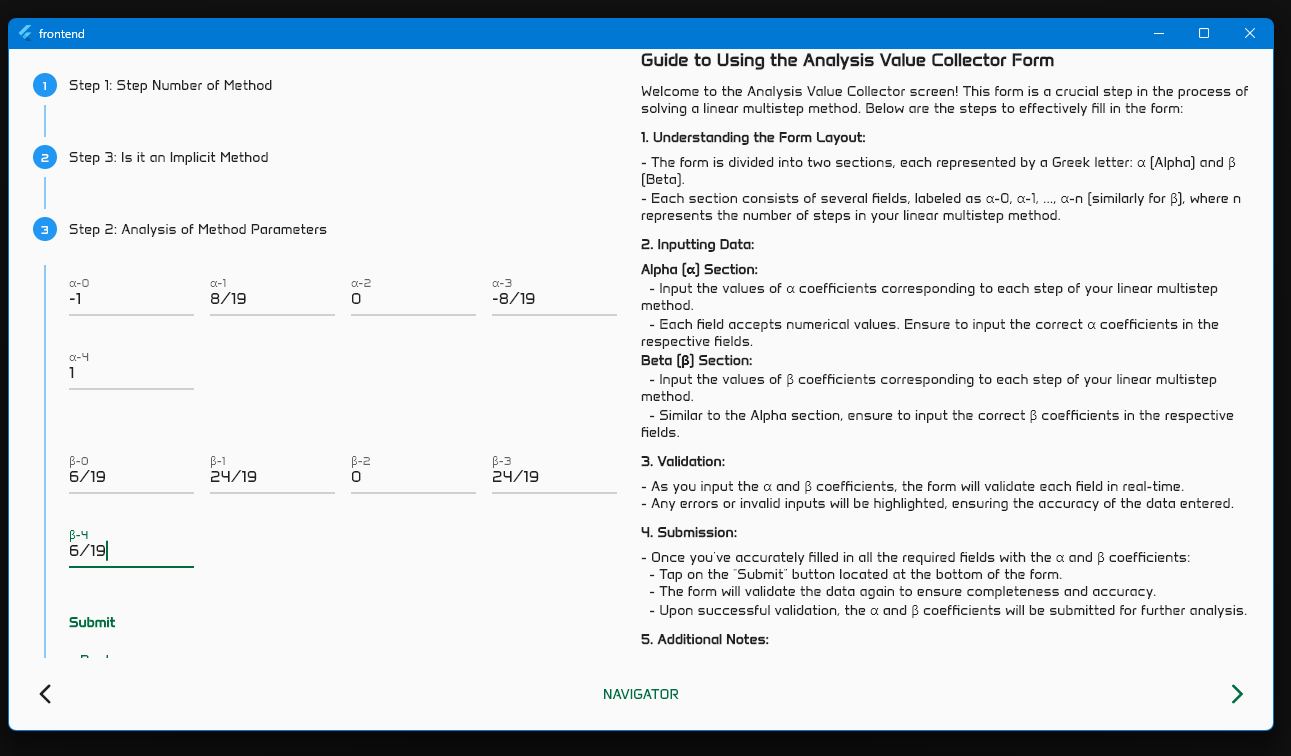
\includegraphics[width=1\textwidth]{chapters/4/image/1.png}
    \caption{$\alpha$ $\beta$ - value collector}
\end{figure}

\begin{figure}[htbp]
    \centering
    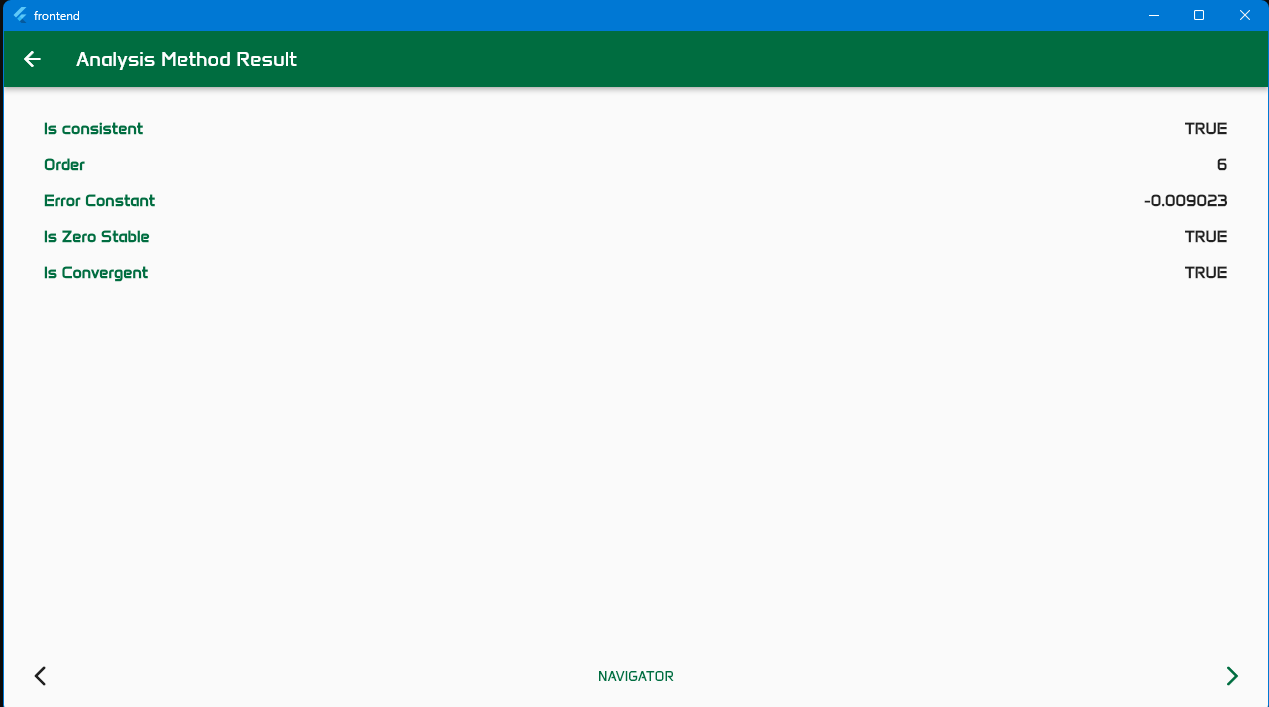
\includegraphics[width=1\textwidth]{chapters/4/image/2.png}
    \caption{Result of Quade's method analysis}
\end{figure}

\newpage

\subsection{Adams Family}
\begin{table}[h!]
    \centering
    \begin{tabularx}{\textwidth}{|c|c|c|X|}
    \hline
    \textbf{Method} & \textbf{Steps} & \textbf{Error Constant} & \textbf{$\beta$ Coefficients} \\
    \hline
    Adams-Bashforth & 2 & $\frac{5}{12}$ & $\beta_1 = \frac{3}{2}, \beta_0 = -\frac{1}{2}$ \\
    \hline
    Adams-Bashforth & 4 & $\frac{251}{720}$ & $\beta_3 = \frac{55}{24}, \beta_2 = -\frac{59}{24}, \beta_1 = \frac{37}{24}, \beta_0 = -\frac{9}{24}$ \\
    \hline
    Adams-Bashforth & 6 & $\frac{19087}{60480}$ & $\beta_5 = \frac{4277}{1440}, \beta_4 = -\frac{7923}{1440}, \beta_3 = \frac{9982}{1440}, \beta_2 = -\frac{7298}{1440}, \beta_1 = \frac{2877}{1440}, \beta_0 = -\frac{475}{1440}$ \\
    \hline
    Adams-Moulton & 3 & $\frac{1}{24}$ & $\beta_0 = \frac{5}{12}, \beta_1 = \frac{2}{3}, \beta_2 = -\frac{1}{12}$ \\
    \hline
    Adams-Moulton & 7 & $\frac{36799}{120960}$ & $\beta_0 = \frac{198721}{60480}, \beta_1 = \frac{18637}{2520}, \beta_2 = -\frac{235183}{20160}, \beta_3 = \frac{10754}{945}, \beta_4 = -\frac{135713}{20160}, \beta_5 = \frac{5603}{2520}, \beta_6 = -\frac{19087}{60480}$ \\
    \hline
    \end{tabularx}
    \caption{Adams-Bashforth and Adams-Moulton Methods with Error Constants and $\beta$ Coefficients}
    \label{table:adams_methods}
    \end{table}
The table (4.1) shows the Error constant for The Adams-Bashforth 2,4, and 6 Step, and also that of the Adams-Moulton 3 and 7 step.

Using the JF-Solver we obtain the same result

\begin{figure}[htbp]
    \centering
    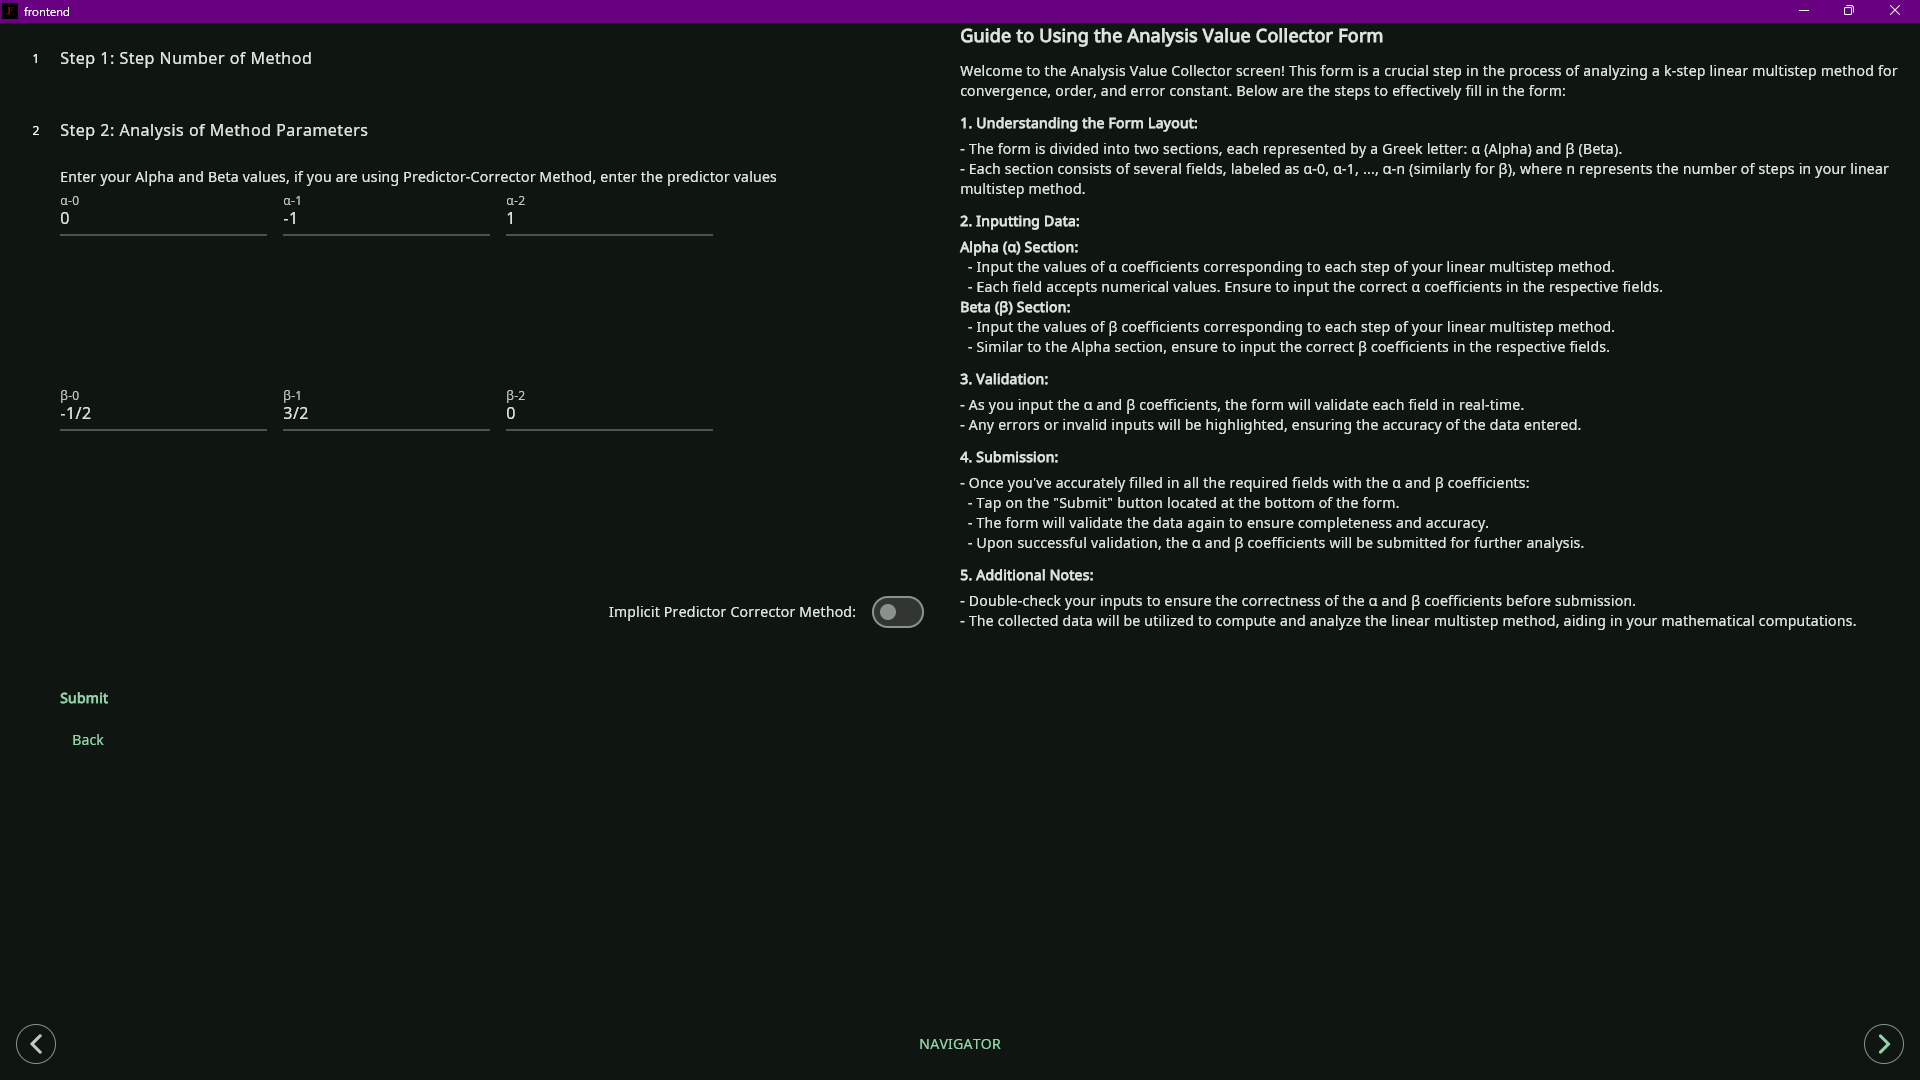
\includegraphics[width=1\textwidth]{chapters/4/image/ab(2)a.png}
    \caption{$\alpha$ $\beta$ - value collector for AB(2) method}
\end{figure}

\begin{figure}[htbp]
    \centering
    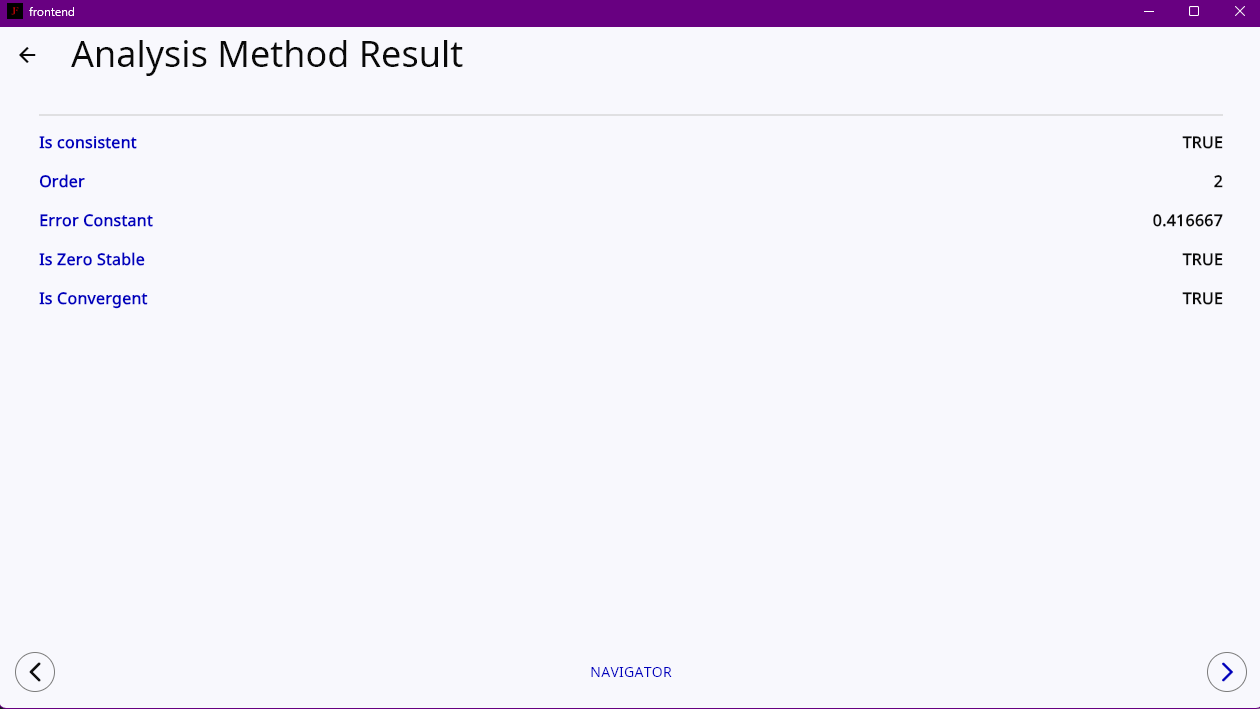
\includegraphics[width=1\textwidth]{chapters/4/image/ab(2)b.png}
    \caption{Results of the AB(2) method analysis}
\end{figure}

\begin{figure}[htbp]
    \centering
    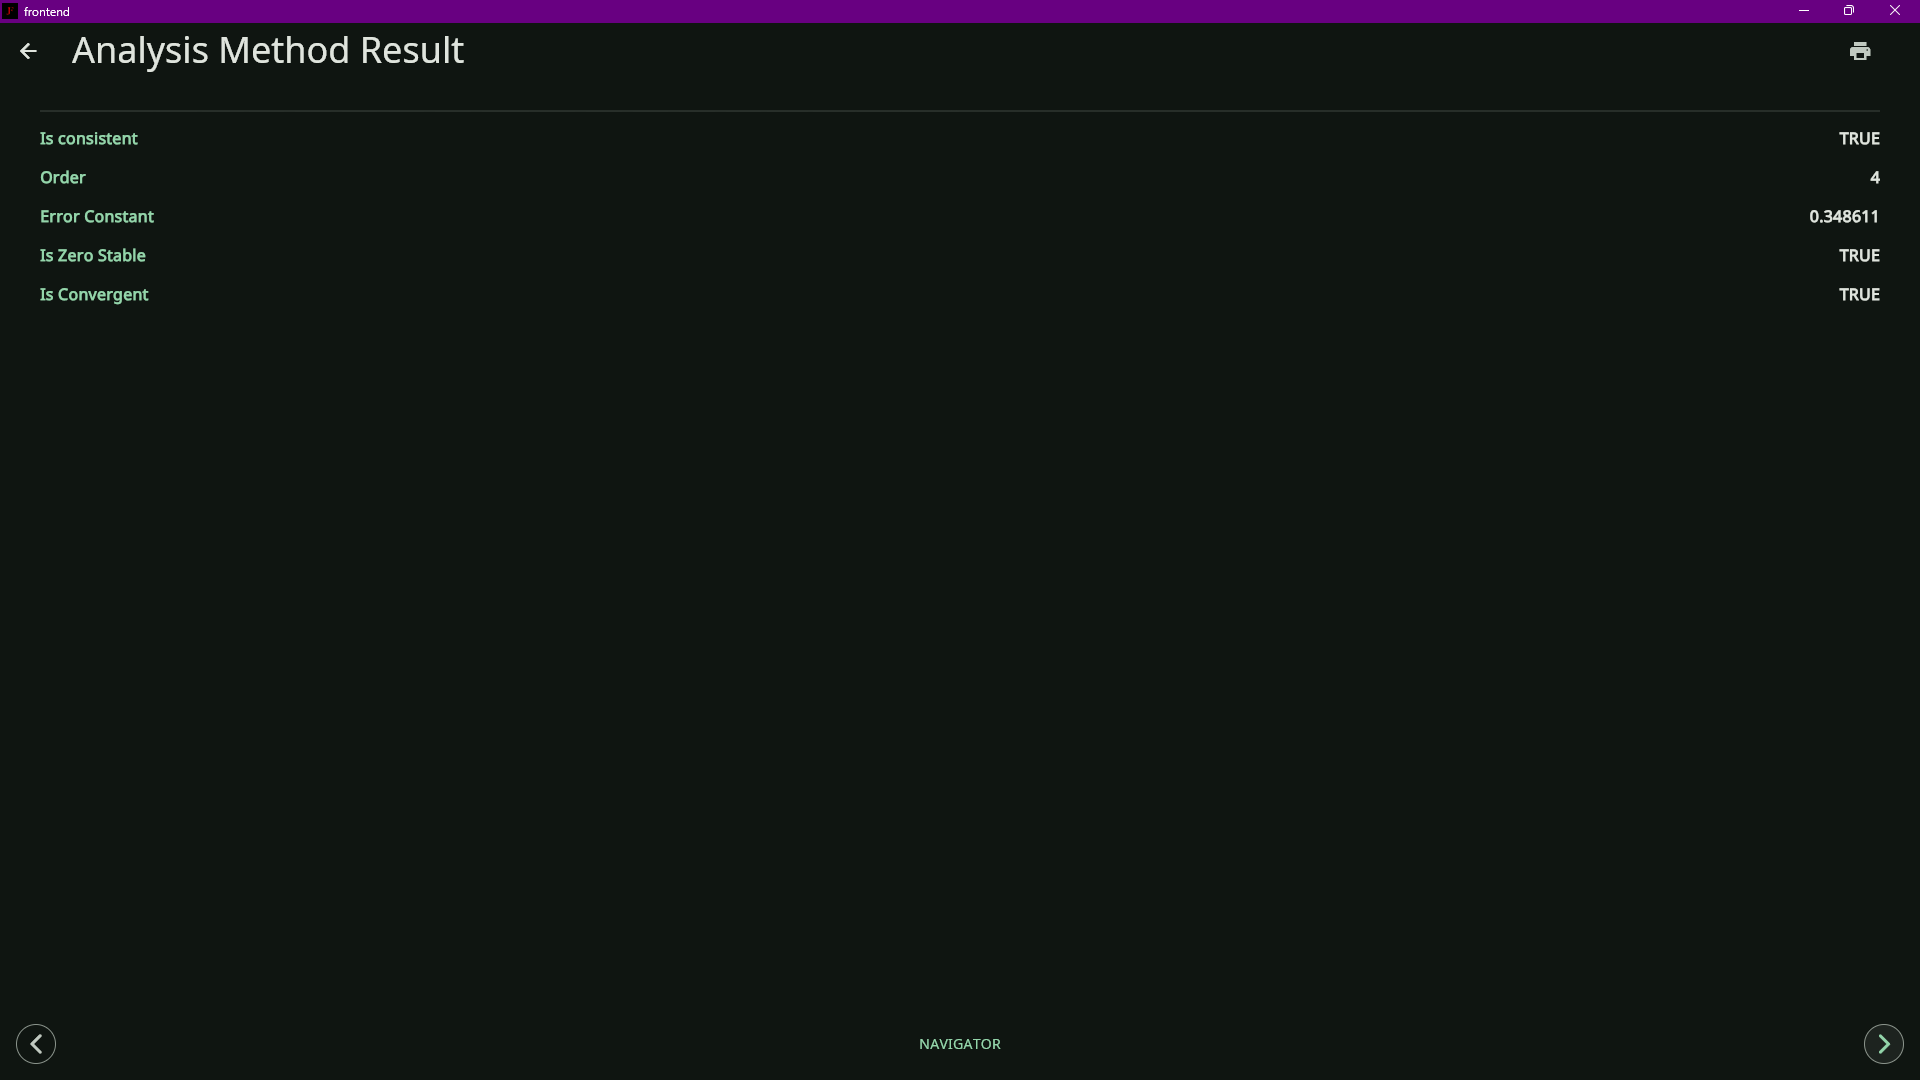
\includegraphics[width=1\textwidth]{chapters/4/image/ab(4)b.png}
    \caption{Results of the AB(4) method analysis}
\end{figure}

\begin{figure}[htbp]
    \centering
    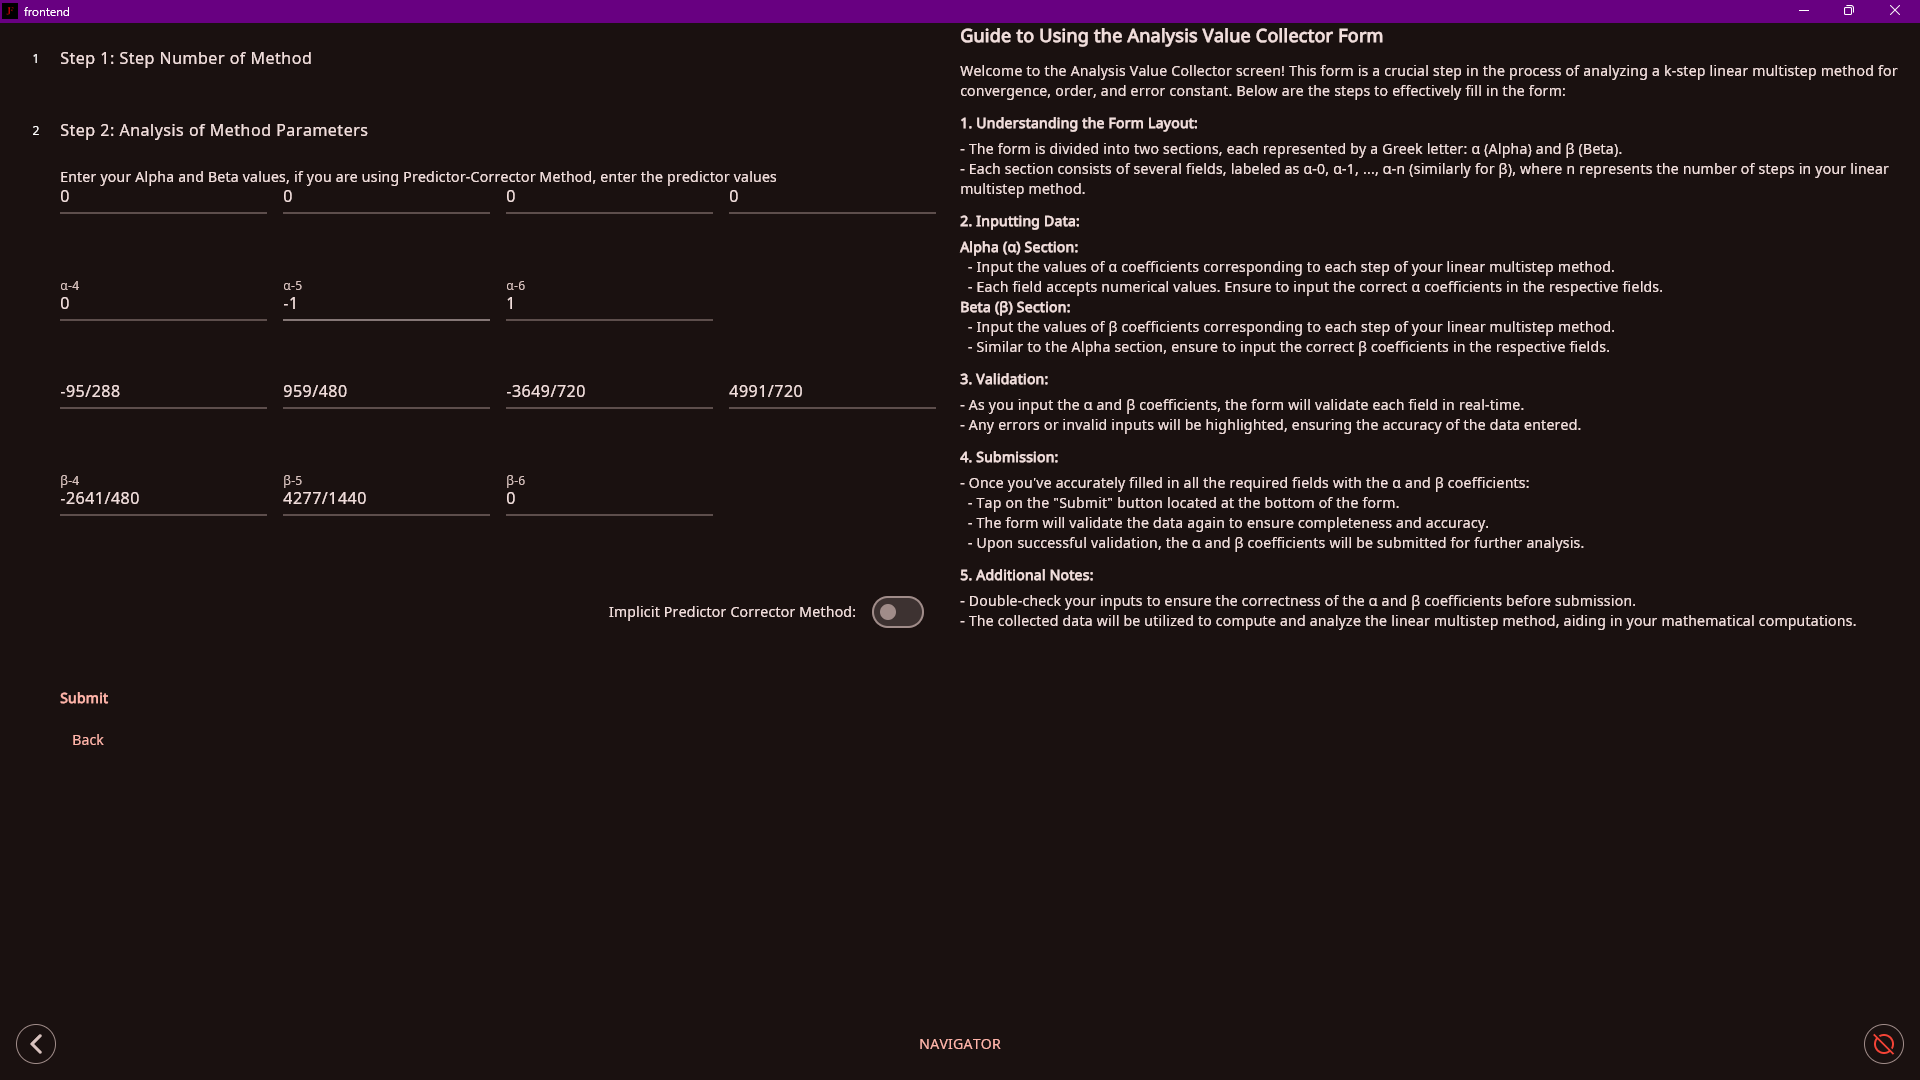
\includegraphics[width=1\textwidth]{chapters/4/image/ab(6)a.png}
    \caption{$\alpha$ $\beta$ - value collector for AB(2) method}
\end{figure}

\begin{figure}[htbp]
    \centering
    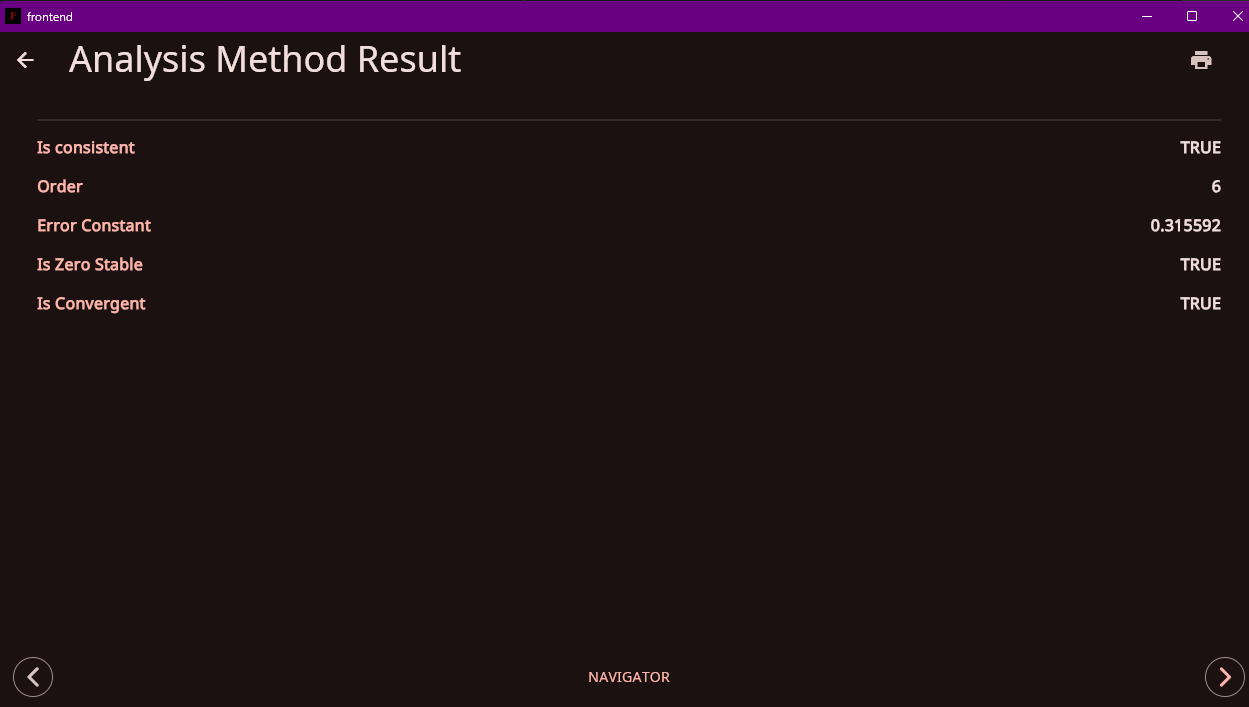
\includegraphics[width=1\textwidth]{chapters/4/image/ab(6).png}
    \caption{Results of the AB(2) method analysis}
\end{figure}


For the Implicit case, that is the Adam Moulton:

\begin{figure}[htbp]
    \centering
    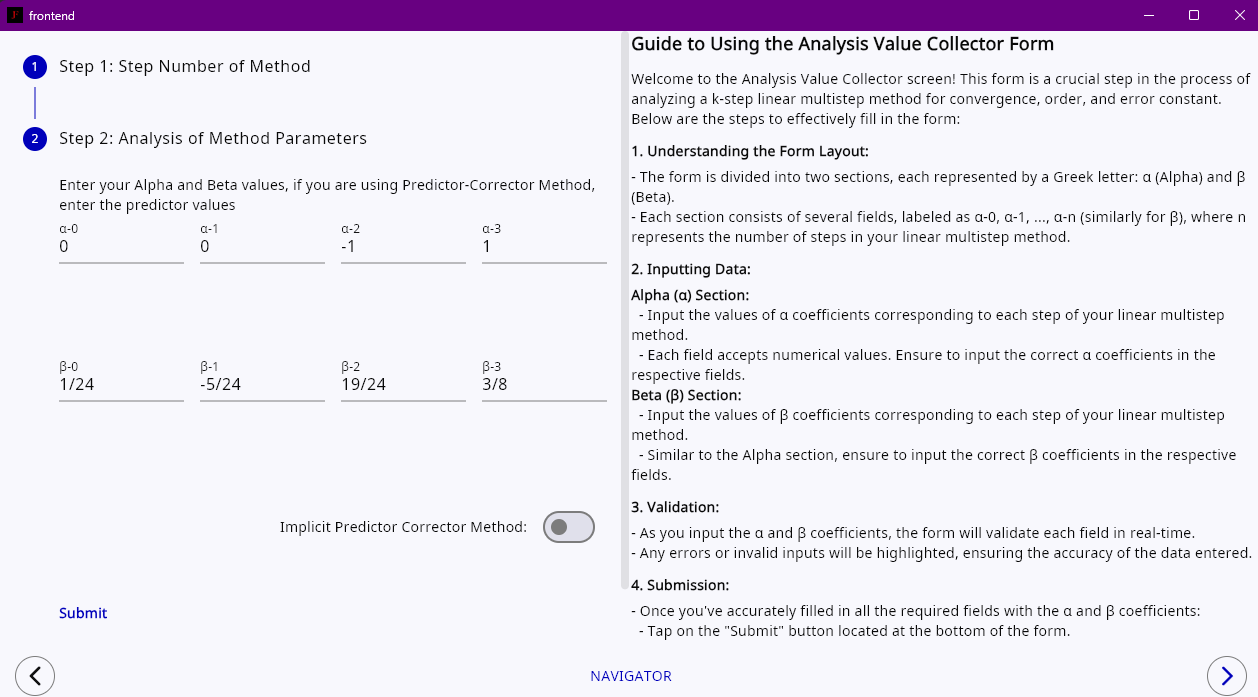
\includegraphics[width=1\textwidth]{chapters/4/image/am(3)a.png}
    \caption{$\alpha$ $\beta$ - value collector for AM(3) method}
\end{figure}

\begin{figure}[htbp]
    \centering
    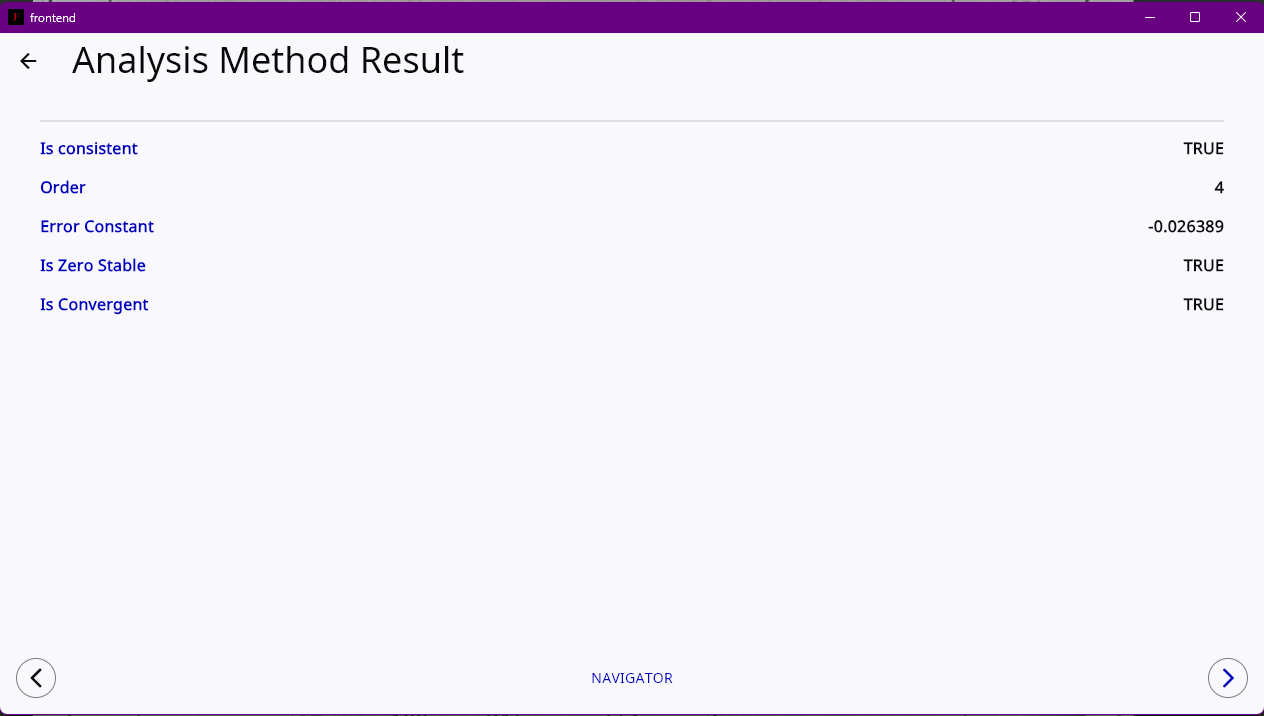
\includegraphics[width=1\textwidth]{chapters/4/image/am(3)b.png}
    \caption{Results of the AM(3) method analysis}
\end{figure}

\begin{figure}[htbp]
    \centering
    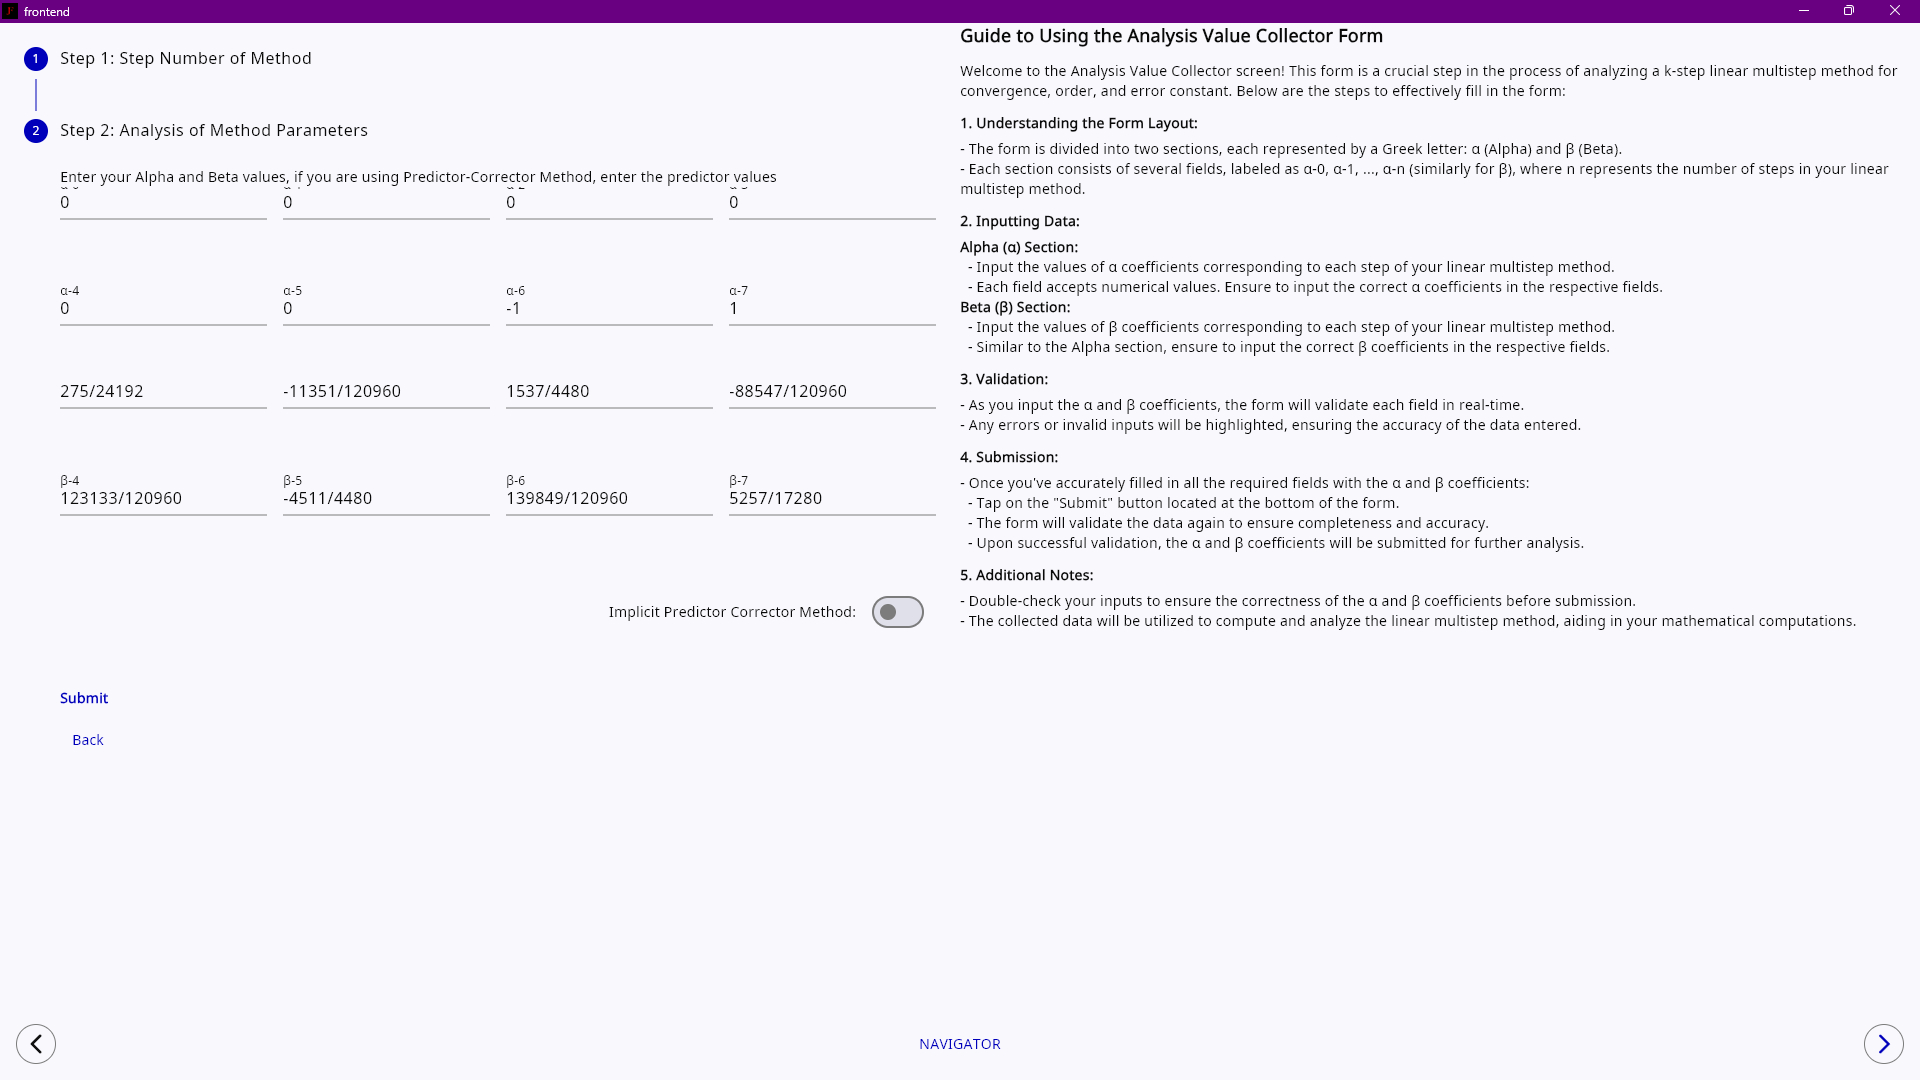
\includegraphics[width=1\textwidth]{chapters/4/image/am(7)a.png}
    \caption{$\alpha$ $\beta$ - value collector for AM(7) method}
\end{figure}

\begin{figure}[htbp]
    \centering
    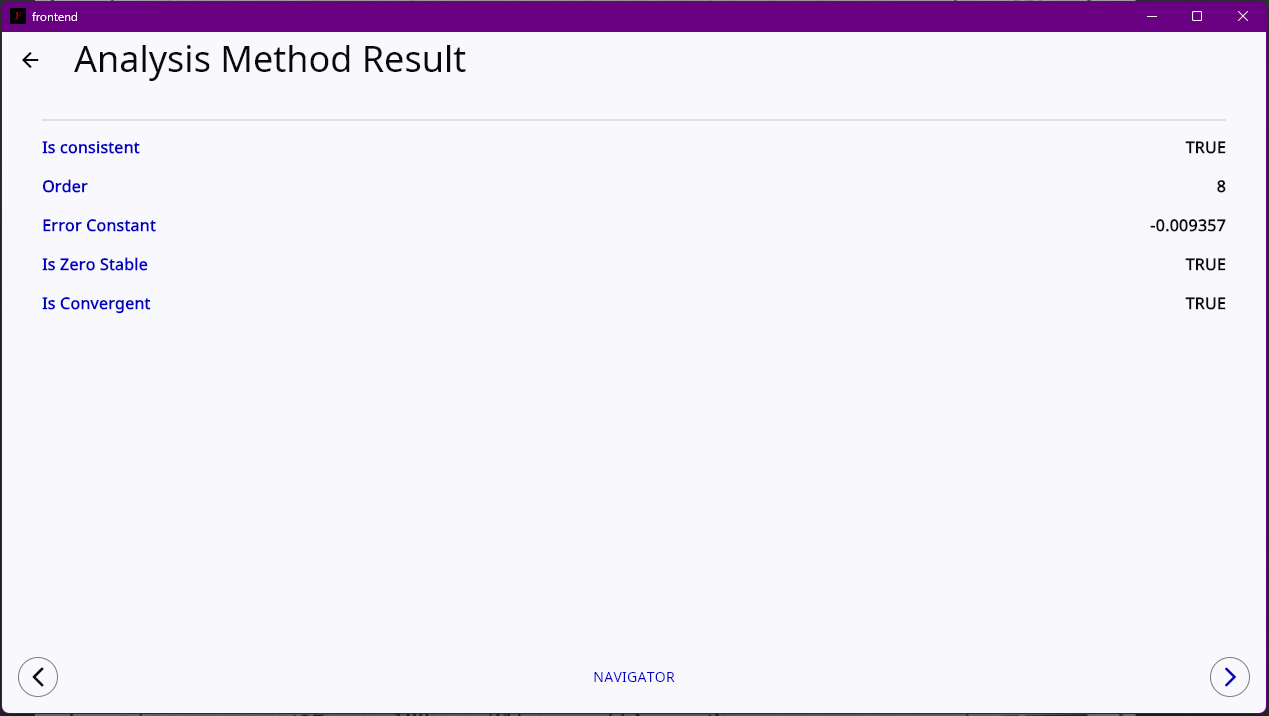
\includegraphics[width=1\textwidth]{chapters/4/image/am(7)b.png}
    \caption{Results of the AM(7) method analysis}
\end{figure}



\newpage


\subsection{3-Step Backward Differentiation Formula}

The 3-Step Backward Differentiation Formula is given as:

\[y_{n+3} = \frac{18}{11} y_{n+2} - \frac{9}{11} y_{n+1} + \frac{2}{11} y_n + \frac{6}{11} h f_{n+3}\]


from the above equation, we can see that the method is a 3-step method,


where:
\[
\begin{aligned}&\alpha_0 &= -\frac{2}{11}, \alpha_1 = \frac{9}{11}, \alpha_2 = -\frac{18}{11}, \alpha_3 = 1 \\
&\beta_0 &= 0, \beta_1 = 0, \beta_2 = 0, \beta_3 = \frac{6}{11}
\end{aligned}
\]

in other to determine the order of the 3-Step BDF's method, we use (3.4), we obtain the following values:

\begin{align}
    c_0 &= \sum_{i=0}^{3} \alpha_i = -\frac{2}{11} + \frac{9}{11} - \frac{18}{11} + 1 = 0 \\
    c_1 &= \sum_{i=0}^{3} (i\alpha_i - \beta_i) = 0 \cdot \alpha_0 + 1 \cdot \alpha_1 + 2 \cdot \alpha_2 + 3 \cdot \alpha_3 - (\beta_0 + \beta_1 + \beta_2 + \beta_3) \nonumber \\
    &= 0 + 1 \cdot \frac{9}{11} + 2 \cdot \left(-\frac{18}{11}\right) + 3 \cdot 1 - \left(0 + 0 + 0 + \frac{6}{11}\right) \nonumber \\
    &= \frac{9}{11} - \frac{36}{11} + 3 - \frac{6}{11} = 0 \\
    c_2 &= \sum_{i=0}^{3} \left(\frac{i^2}{2!} \alpha_i - i \beta_i \right) = \left(\frac{0^2}{2!} \alpha_0 - 0 \cdot \beta_0\right) + \left(\frac{1^2}{2!} \alpha_1 - 1 \cdot \beta_1\right) + \left(\frac{2^2}{2!} \alpha_2 - 2 \cdot \beta_2\right) + \left(\frac{3^2}{2!} \alpha_3 - 3 \cdot \beta_3\right) \nonumber \\
    &= 0 + \frac{1}{2} \cdot \frac{9}{11} - 0 + \frac{4}{2} \cdot \left(-\frac{18}{11}\right) - 0 + \frac{9}{2} \cdot 1 - \frac{18}{11} \nonumber \\
    &= \frac{9}{22} - \frac{36}{11} + \frac{9}{2} - \frac{18}{11} = 0 \\
    c_3 &= \sum_{i=0}^{3} \left(\frac{i^3}{3!} \alpha_i - \frac{i^2}{2!} \beta_i \right) = \left(\frac{0^3}{3!} \alpha_0 - \frac{0^2}{2!} \beta_0\right) + \left(\frac{1^3}{3!} \alpha_1 - \frac{1^2}{2!} \beta_1\right) + \left(\frac{2^3}{3!} \alpha_2 - \frac{2^2}{2!} \beta_2\right) + \left(\frac{3^3}{3!} \alpha_3 - \frac{3^2}{2!} \beta_3\right) \nonumber \\
    &= 0 + \frac{1}{6} \cdot \frac{9}{11} - \frac{1}{2} \cdot 0 + \frac{8}{6} \cdot \left(-\frac{18}{11}\right) - \frac{4}{2} \cdot 0 + \frac{27}{6} \cdot 1 - \frac{9}{2} \cdot \frac{6}{11} \nonumber \\
    &= \frac{9}{66} - \frac{144}{66} + \frac{27}{6} - \frac{54}{11} = 0 \\
    c_4 &= \sum_{i=0}^{3} \left(\frac{i^4}{4!} \alpha_i - \frac{i^3}{3!} \beta_i \right) = \left(\frac{0^4}{4!} \alpha_0 - \frac{0^3}{3!} \beta_0 \right) + \left(\frac{1^4}{4!} \alpha_1 - \frac{1^3}{3!} \beta_1 \right) + \left(\frac{2^4}{4!} \alpha_2 - \frac{2^3}{3!} \beta_2 \right) + \left(\frac{3^4}{4!} \alpha_3 - \frac{3^3}{3!} \beta_3 \right) \nonumber \\
    &= 0 + \frac{1}{24} \cdot \frac{9}{11} - \frac{1}{6} \cdot 0 + \frac{16}{24} \cdot \left(-\frac{18}{11}\right) - \frac{8}{6} \cdot 0 + \frac{81}{24} \cdot 1 - \frac{27}{6} \cdot \frac{6}{11} \nonumber \\
    &= \frac{9}{264} - \frac{288}{264} + \frac{81}{24} - \frac{162}{22} = -\frac{3}{22} = - 0.13636364
\end{align}




The characteristic polynomial \(P(z)\) associated with the BDF-3 method is given by:

\begin{equation}
    P(z) = 11z^3 - 18z^2 + 9z - 2  
\end{equation}



Solving the Algebraic Equation 

\begin{eqnarray}
    11z^3 - 18z^2 + 9z - 2 = 0 \\
    11z^3 - 18z^2 + 9z - 2 = (z - 1)(11z^2 - 7z + 2) \\    
    11z^2 - 7z + 2 = 0 \\
    (z - 1) = 0 \\
    z = \frac{7 \pm \sqrt{(-7)^2 - 4(11)(2)}}{2(11)} = \frac{7 \pm \sqrt{49 - 88}}{22} = \frac{7 \pm i\sqrt{39}}{22} 
\end{eqnarray}

Therefore, the roots of the polynomial \(11z^3 - 18z^2 + 9z - 2 = 0\) are:

\begin{eqnarray}
    z = 1 \\
    z = \frac{7 + i\sqrt{39}}{22} \\
    z = \frac{7 - i\sqrt{39}}{22}
\end{eqnarray}
We take the modulus of the roots to check for zero-stability:
\begin{eqnarray}
    |z| = |1| = 1 \\
    |z| = \sqrt{\left(\frac{7}{22}\right)^2 + \left(\frac{\sqrt{39}}{22}\right)^2} = \sqrt{\frac{49}{484} + \frac{39}{484}} = \sqrt{\frac{88}{484}} = \sqrt{\frac{22}{121}} = \frac{\sqrt{22}}{11} < 1 \\
    |z| = \sqrt{\left(\frac{7}{22}\right)^2 + \left(-\frac{\sqrt{39}}{22}\right)^2} = \sqrt{\frac{49}{484} + \frac{39}{484}} = \sqrt{\frac{88}{484}} = \sqrt{\frac{22}{121}} = \frac{\sqrt{22}}{11} < 1
\end{eqnarray}

Using Equation (3.4), we can see that the method is a 3-step method of order 3. The method is consistent since \(c_0 = 0\) and \(c_1 = 0\). Furthermore, the method is zero-stable since the roots of the characteristic equation are all inside the unit circle. Lastly, the method is convergent since the error constant is \(-\frac{3}{22}\) or approximately \(-0.1363634\).

Using the JF-Solver to analyze the 3-step Backward Differentiation Formula (BDF(3)), we obtain the following results as shown below:

\begin{figure}[htbp]
    \centering
    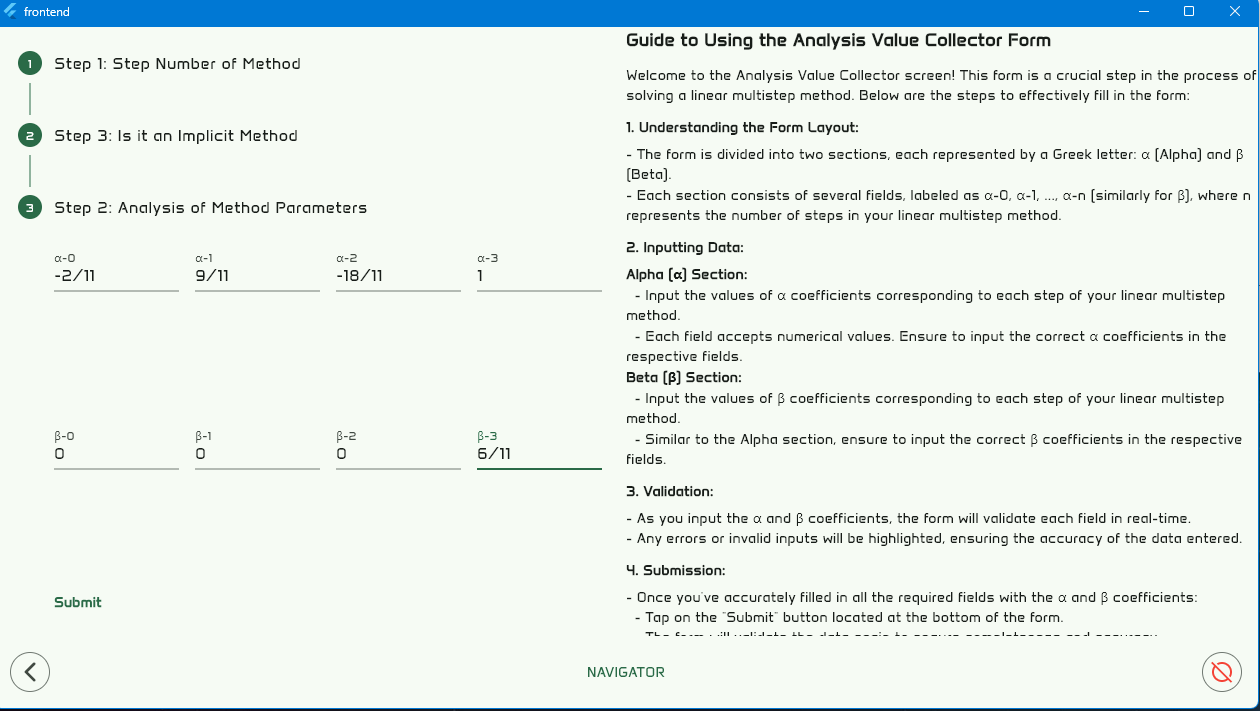
\includegraphics[width=1\textwidth]{chapters/4/image/5.png}
    \caption{$\alpha$ $\beta$ - value collector for 3-step BDF method}
\end{figure}

\begin{figure}[htbp]
    \centering
    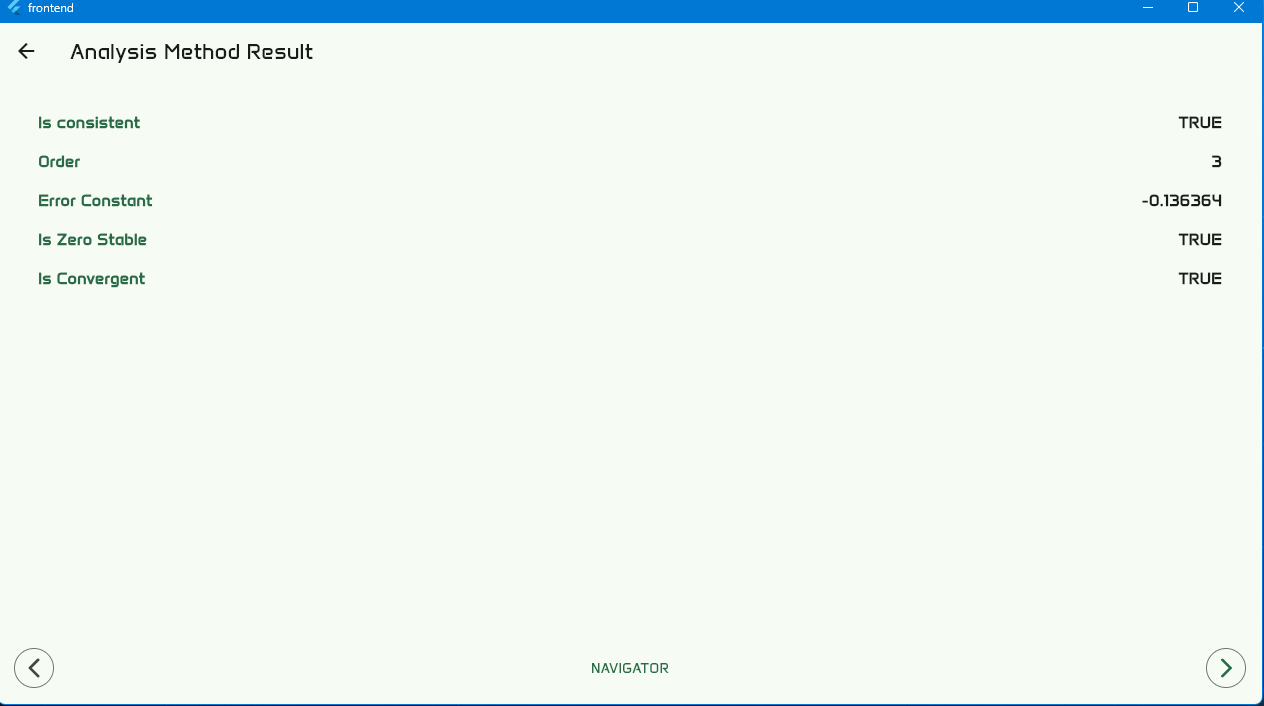
\includegraphics[width=1\textwidth]{chapters/4/image/6.png}
    \caption{Results of the 3-step BDF method analysis}
\end{figure}



Additionally, the JF-Solver software, which was developed as part of this research, has been used to analyze the BDF(3) method. The software successfully replicated the theoretical results, providing the same error constant and stability characteristics. Moreover, the JF-Solver demonstrated superior performance in terms of computation speed and efficiency, making it a valuable tool for numerical analysis of differential equations.


%! Module 2: Solving Differential Equations

% \newpage
\section{Module 2: Solving Differential Equations}

\subsection{Explicit Method: Adams-Bashforth Method 3-Step Method}
Consider the problem \begin{equation}
    f(x,y) = 3x^2y
\end{equation}, with the initial condition $y(0) = 1$, the step-size also given as $h = 0.1$.

The Adams-Bashforth 3-step method is given as:
\begin{equation}
    y_{n+3}  = y_{n+2} + h \left(\frac{23}{12}f_{n+2} - \frac{4}{3}f_{n+1} + \frac{5}{12}f_{n}\right)
\end{equation}

The exact solution to the problem is given as:
\begin{equation}
    y(x) = e^{x^3}
\end{equation}




\begin{table}[htbp]
    \centering
    \begin{tabular}{|c|c|c|c|}
        \hline
        Step $n$ & Adams-Bashforth 3-step Method & JF-Solver & Exact Value \\
        \hline
        $y_0$ & 1.000000 & 1.000000 & 1.000000 \\
        $y_1$ & 1.001000 & 1.001000 & 1.001001 \\
        $y_2$ & 1.008032 & 1.008032 & 1.008032 \\
        $y_3$ & 1.027213 & 1.027213 & 1.027398 \\
        $y_4$ & 1.065494 & 1.065494 & 1.066492 \\
        $y_5$ & 1.131580 & 1.131580 & 1.133148 \\
        $y_6$ & 1.237609 & 1.237609 & 1.241857 \\
        $y_7$ & 1.401946 & 1.401946 & 1.409637 \\
        $y_8$ & 1.654090 & 1.654090 & 1.669859 \\
        $y_9$ & 2.043706 & 2.043706 & 2.073784 \\
        \hline
    \end{tabular}
    \caption{Comparison of Results: Adams-Bashforth 3-step Method, JF-Solver, and Exact Values}
    \label{tab:comparison}
\end{table}


The table illustrates the numerical values obtained at each step $n$. The Adams-Bashforth 3-step method and the JF-Solver results are compared against the exact solution $y = e^{x^3}$.

The images below shows that output of the JF-Solver:

\begin{figure}[htbp]
    \centering
    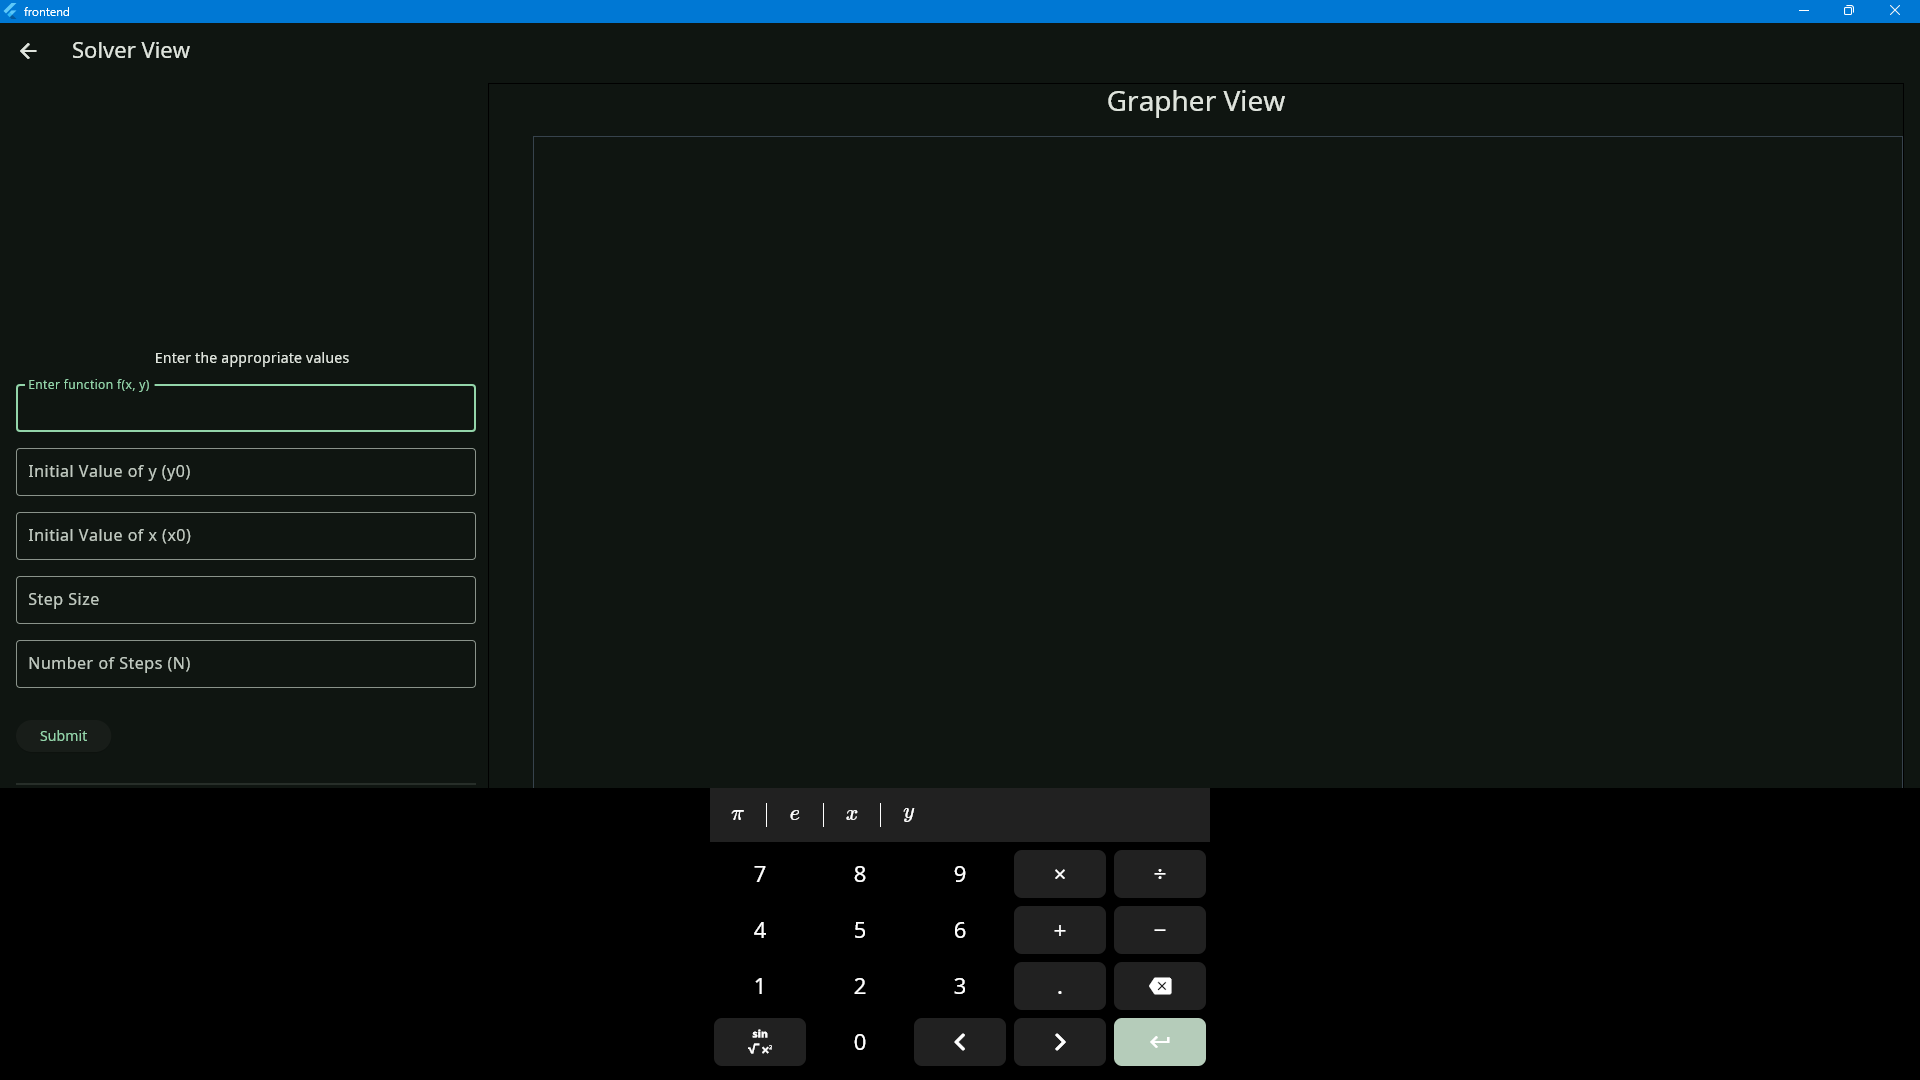
\includegraphics[width=1\textwidth]{chapters/4/image/solver_3.png}
    \caption{The JF-Solver view}
\end{figure}

\begin{figure}[htbp]
    \centering
    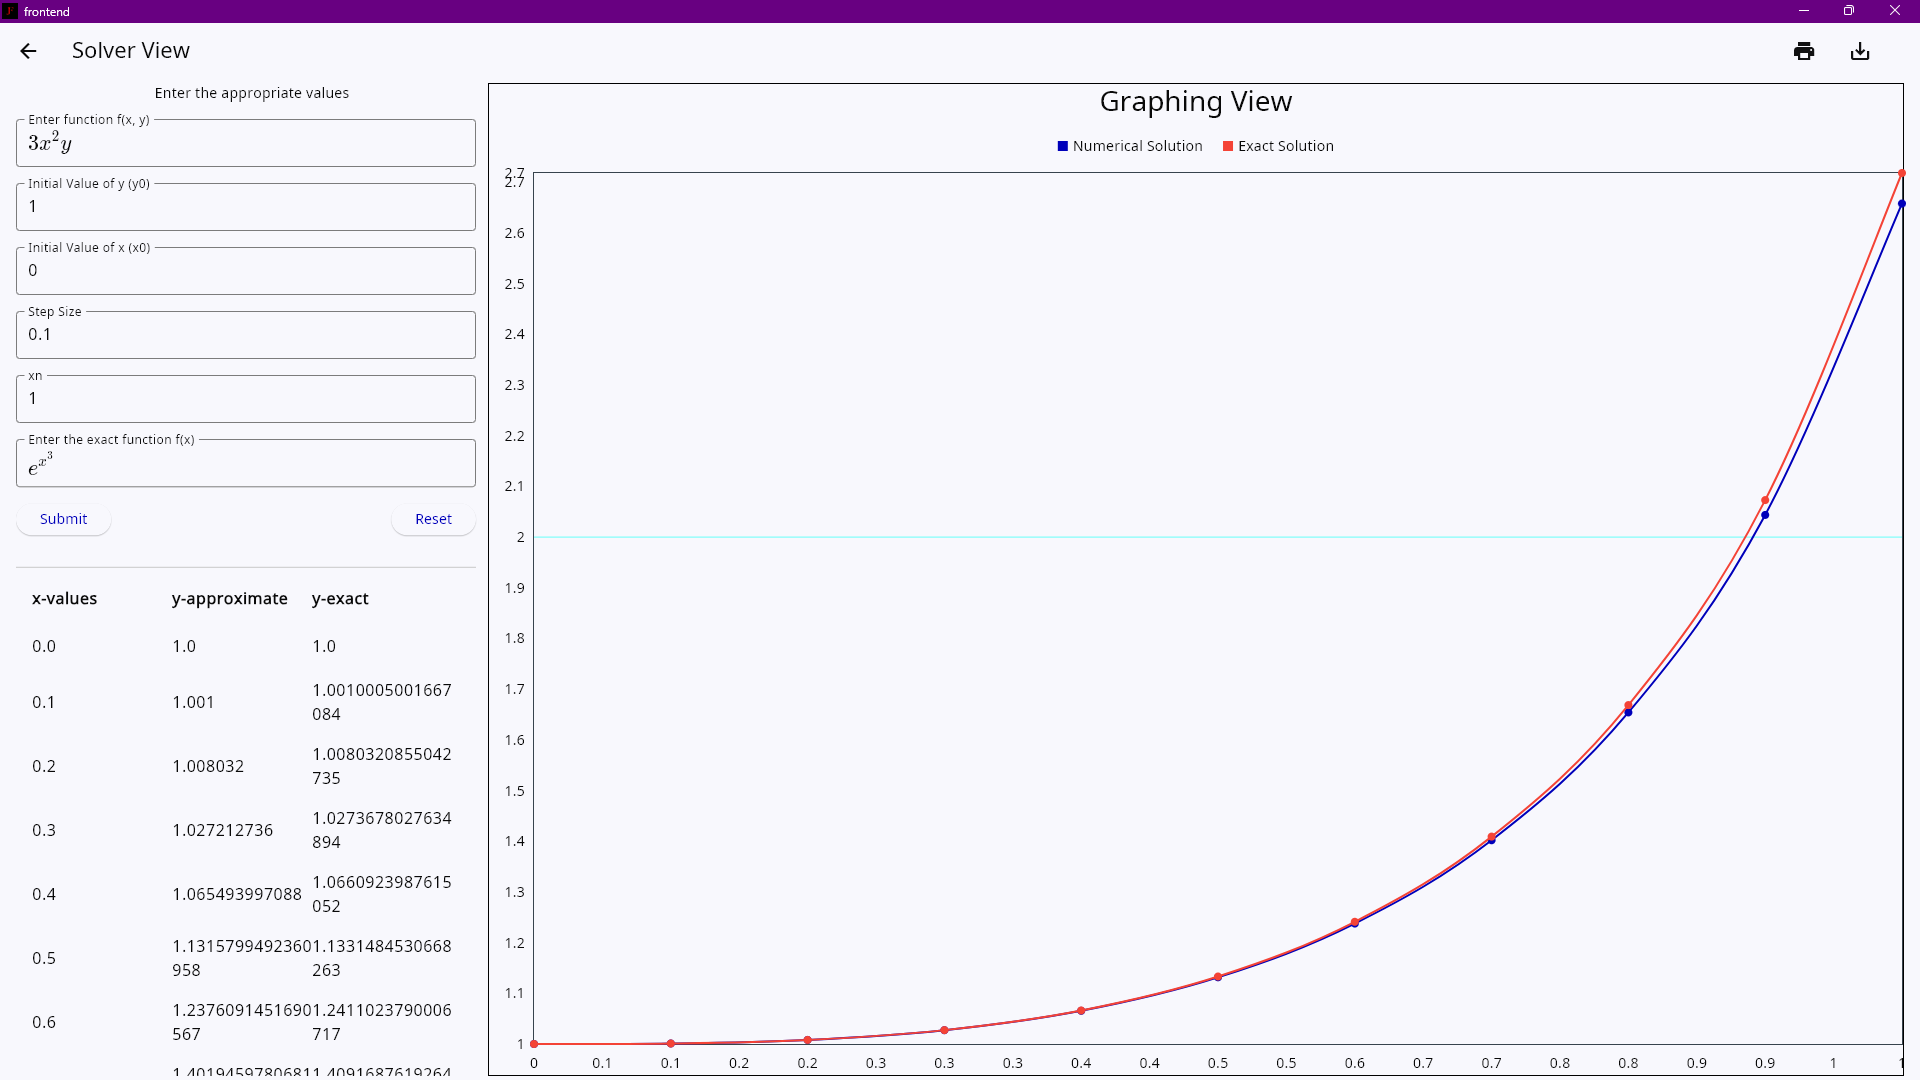
\includegraphics[width=1\textwidth]{chapters/4/image/solver_2.png}
    \caption{output result of the JF-Solver for $(4.30)$ }
\end{figure}


\newpage
From the comparison, it is evident that both the Adams-Bashforth 3-step method and the JF-Solver produce results that closely approximate the exact solution. The JF-Solver results are rounded to six decimal places, showing a high degree of accuracy.

This comparison demonstrates the effectiveness, accuracy, and reliability of the JF-Solver in approximating the solution of explicit differential equations using the Linear Multistep Method (LMM) given. The application works by accepting the coefficients of the LMM and then solves the differential equation using these coefficients.

\section{Implicit Method(Predictor-Corrector Algorithm): Adams-Moulton Method 4-Step Method (Non-Stiff problem)}

Consider the problem \begin{equation}
    f(x,y) = x + y
\end{equation}, with the initial condition $y(0) = 0$, the step-size also given as $h = 0.2$.

We use two LMM methods that are of the same order, the predictor method which is an explicit method, and the corrector method which is an Implicit method, for this example, the predictor method is the 4-step Adam Bashforth given as

\begin{equation}
    y_{n+4}  = y_{n+3} + h \left(\frac{55}{24}f_{n+3} - \frac{59}{24}f_{n+2} + \frac{37}{24}f_{n+1} - \frac{9}{24}f_{n}\right)
\end{equation}

The corrector method is the 3-step Adam-Moulton method, which is given as:

\begin{equation}
    y_{n+3}  = y_{n+2} + h \left(\frac{9}{24}f_{n+3} + \frac{19}{24}f_{n+2} - \frac{5}{24}f_{n+1} + \frac{1}{24}f_{n}\right)
\end{equation}

both method are of the same order, that is order 4, this is determined by the JF-Solver, and this is discussed in  (Advanced Engineering Mathematics, Erwin Kreyszig,Table 21.9, Pg 914)

\begin{figure}[htbp]
    \centering
    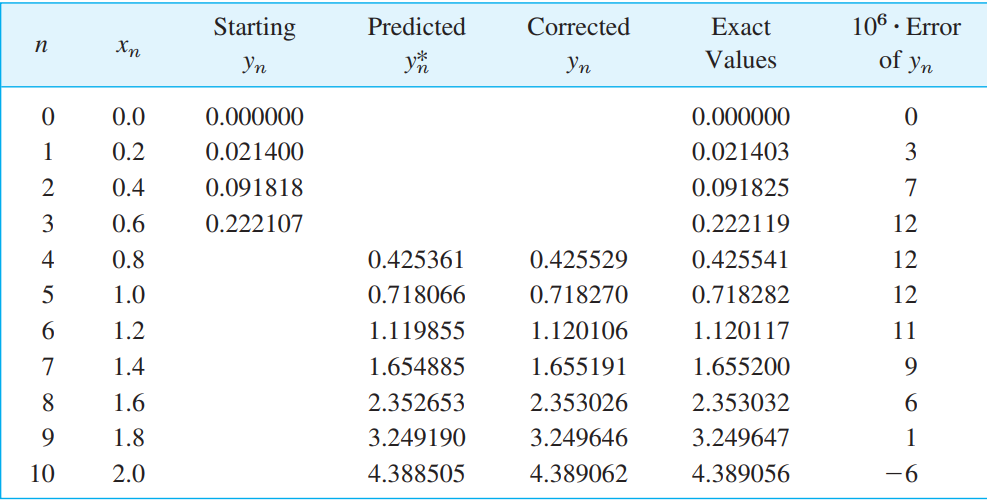
\includegraphics[width=1\textwidth]{chapters/4/image/solver_4.png}
    \caption{Predicted and Corrected Values of $(4.33)$ }
\end{figure}



\begin{figure}[htbp]
    \centering
    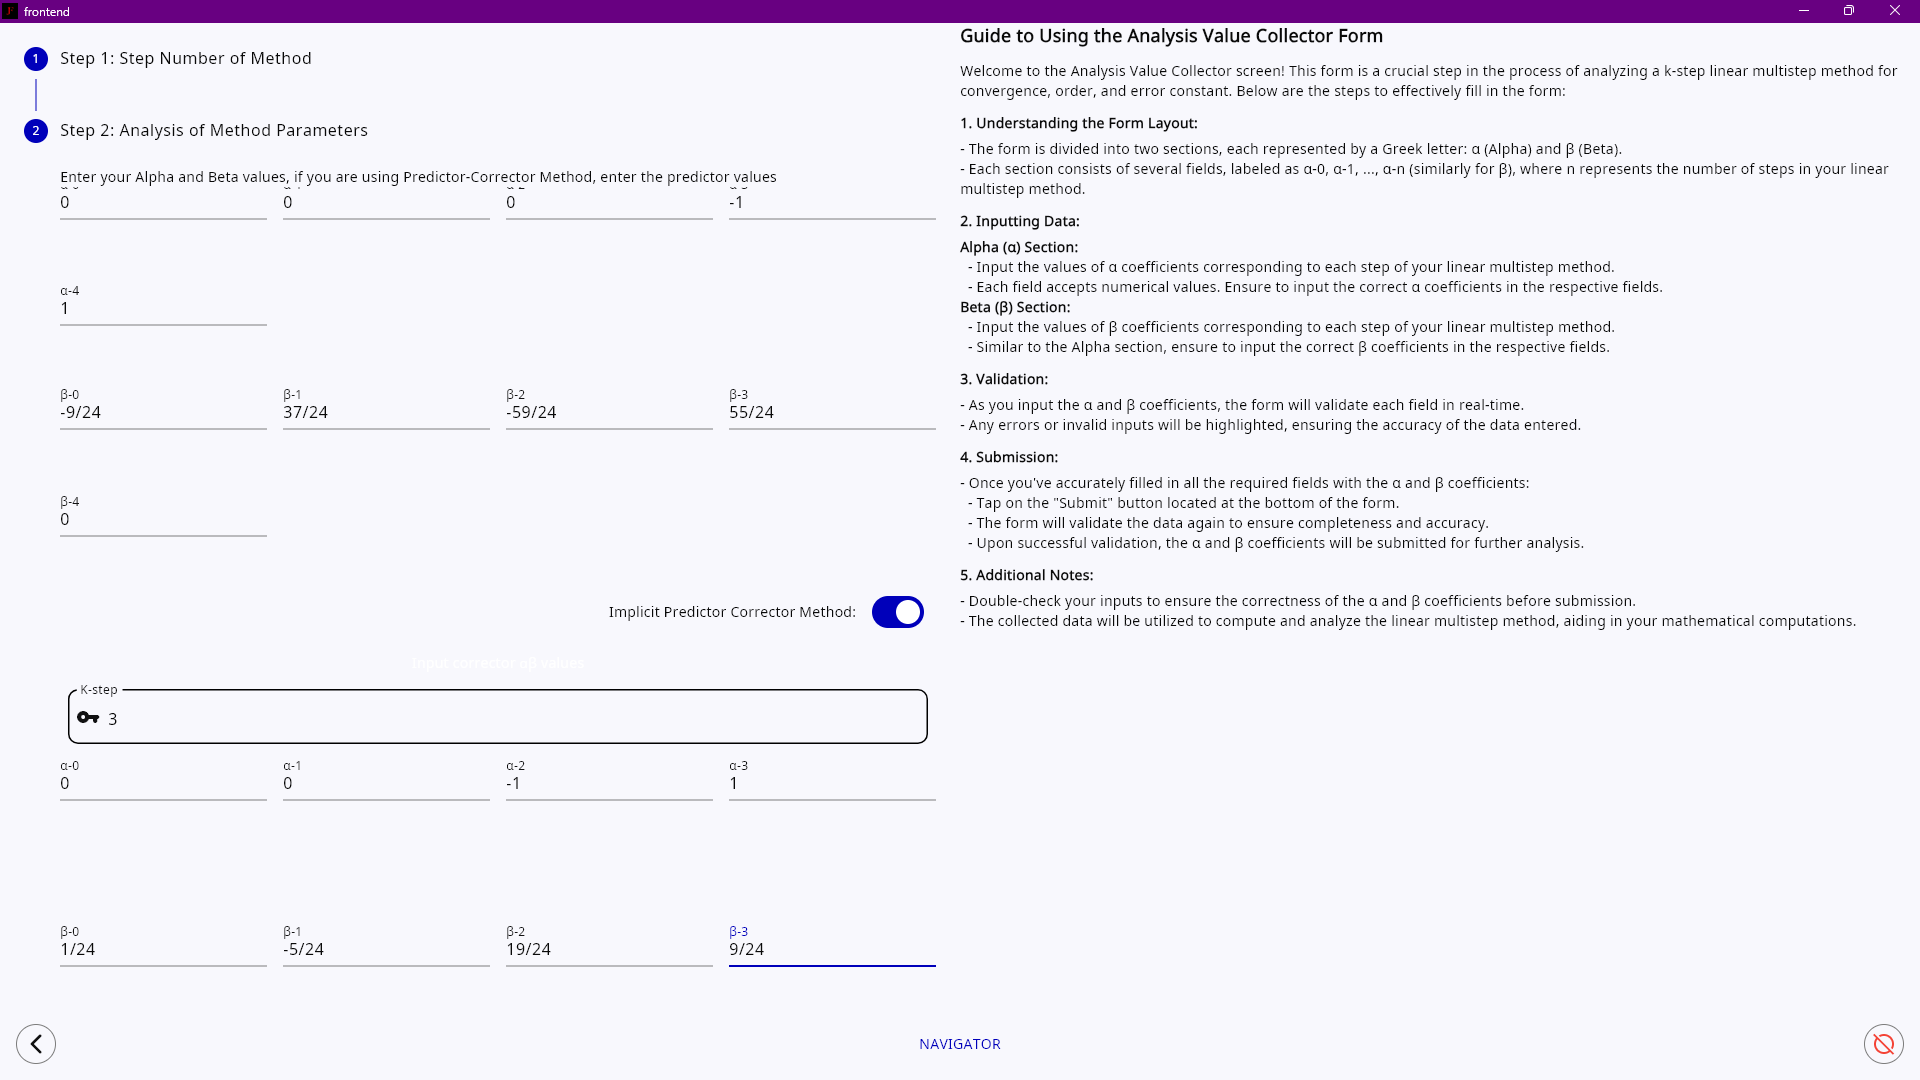
\includegraphics[width=1\textwidth]{chapters/4/image/solver_5.png}
    \caption{entering $\alpha$ and $\beta$ values into the JF-Solver }
\end{figure}


we use the JF-Solver to get the solution $(4.33)$ and also analysis the Predictor-Corrector method  used,we get the following result:


\begin{figure}[htbp]
    \centering
    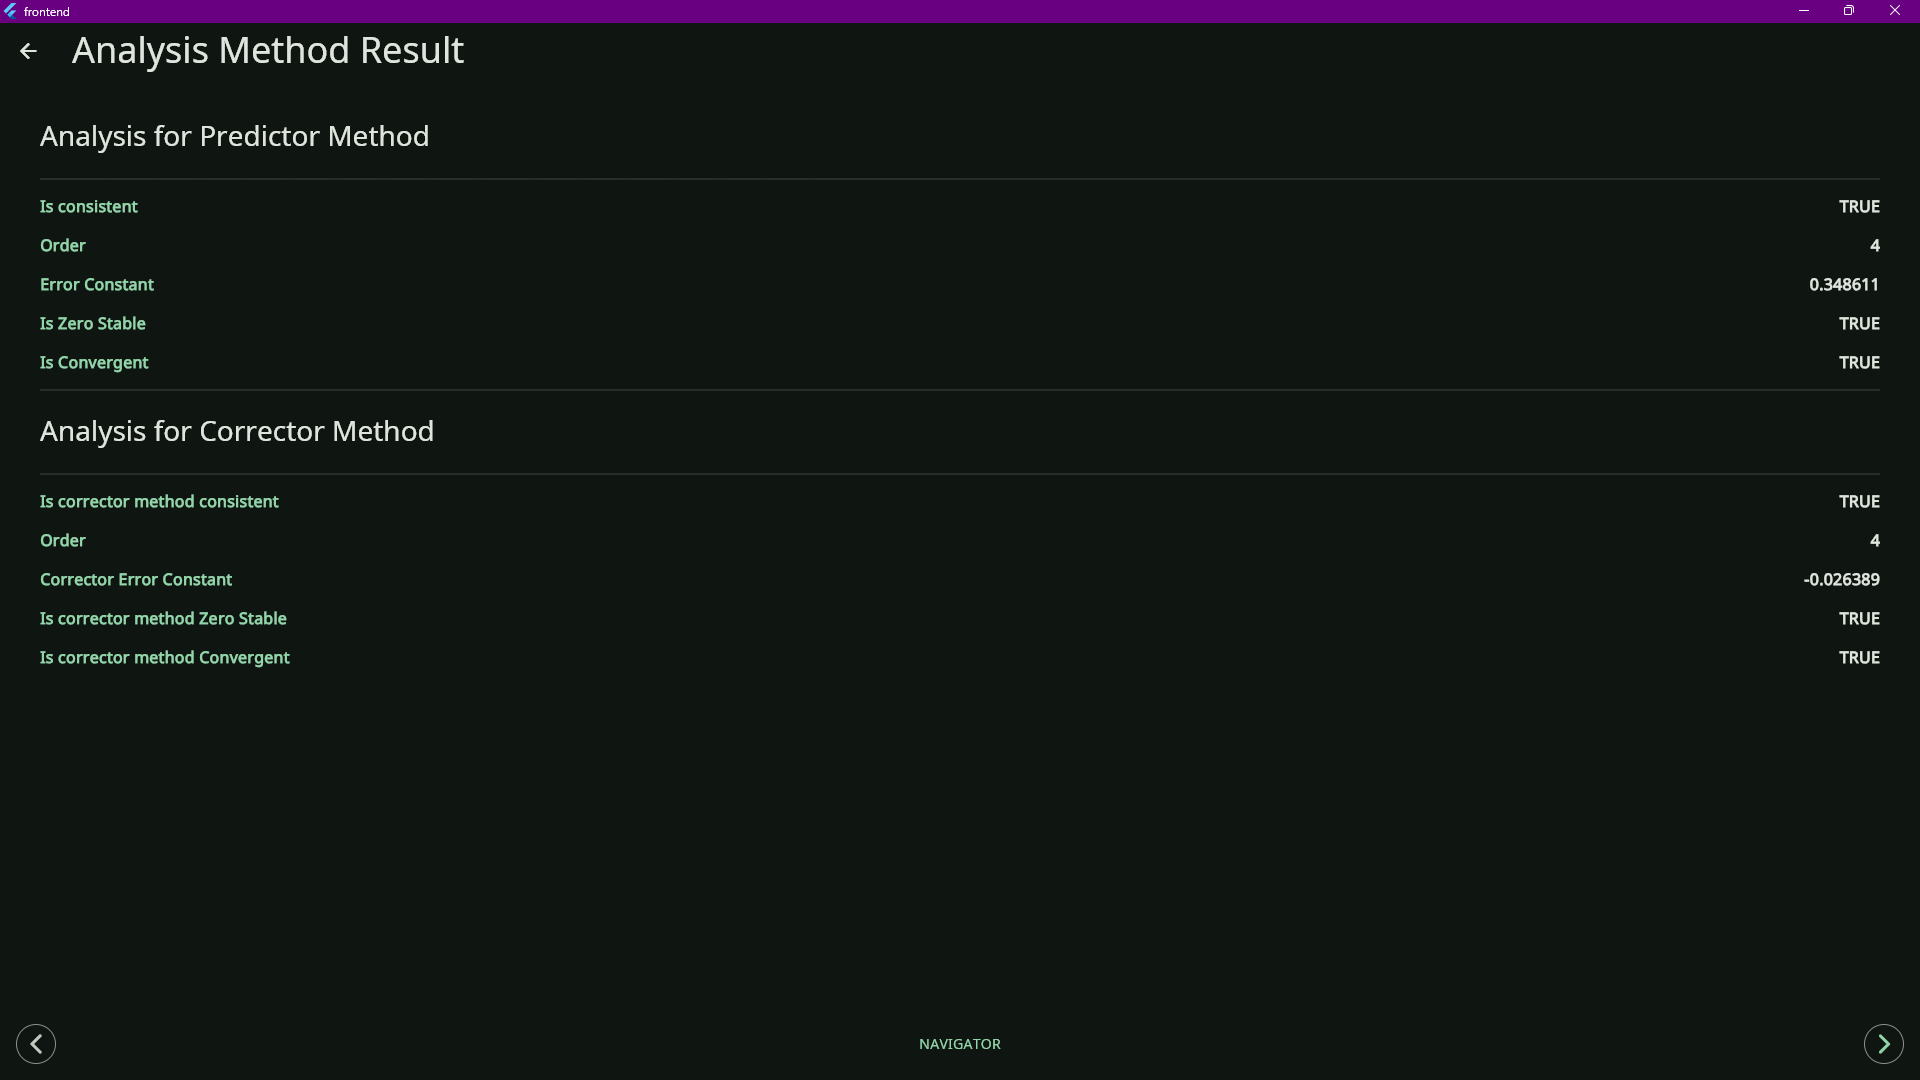
\includegraphics[width=1\textwidth]{chapters/4/image/solver_6.png}
    \caption{Analysis result of $(4.33)$ }
\end{figure}


\begin{figure}[htbp]
    \centering
    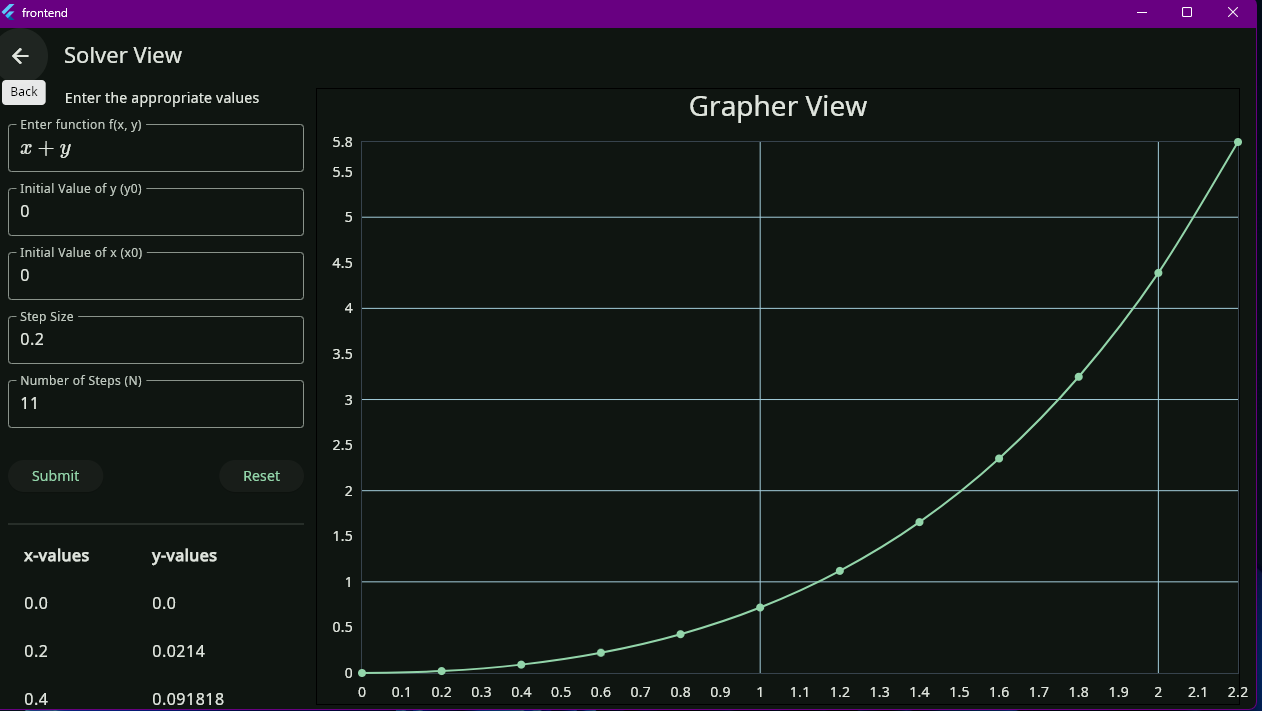
\includegraphics[width=1\textwidth]{chapters/4/image/solver_7.png}
    \caption{solution of $(4.33)$ by JF-Solver}
\end{figure}


\newpage

\section{Implicit Method: 3-Step Backward Differentiation Formula Method (Stiff problem)}


The Dahlquist Test Equation is given as:
\begin{equation}
    y'(x) = Ky(x)
\end{equation}
Where $K$ is a constant, this equation becomes a stiff problem when $K$ is negative. The JF-Solver is used to solve this equation using the 3-step Backward Differentiation Formula Method, which has been proven to be effective for solving stiff problems.

The solver is used to analyze the scheme and to solve the stiff problem:

\begin{equation}
y'(x) = -16y(x)
\end{equation}

The solution to the problem is shown below:

\begin{figure}[htbp]
    \centering
    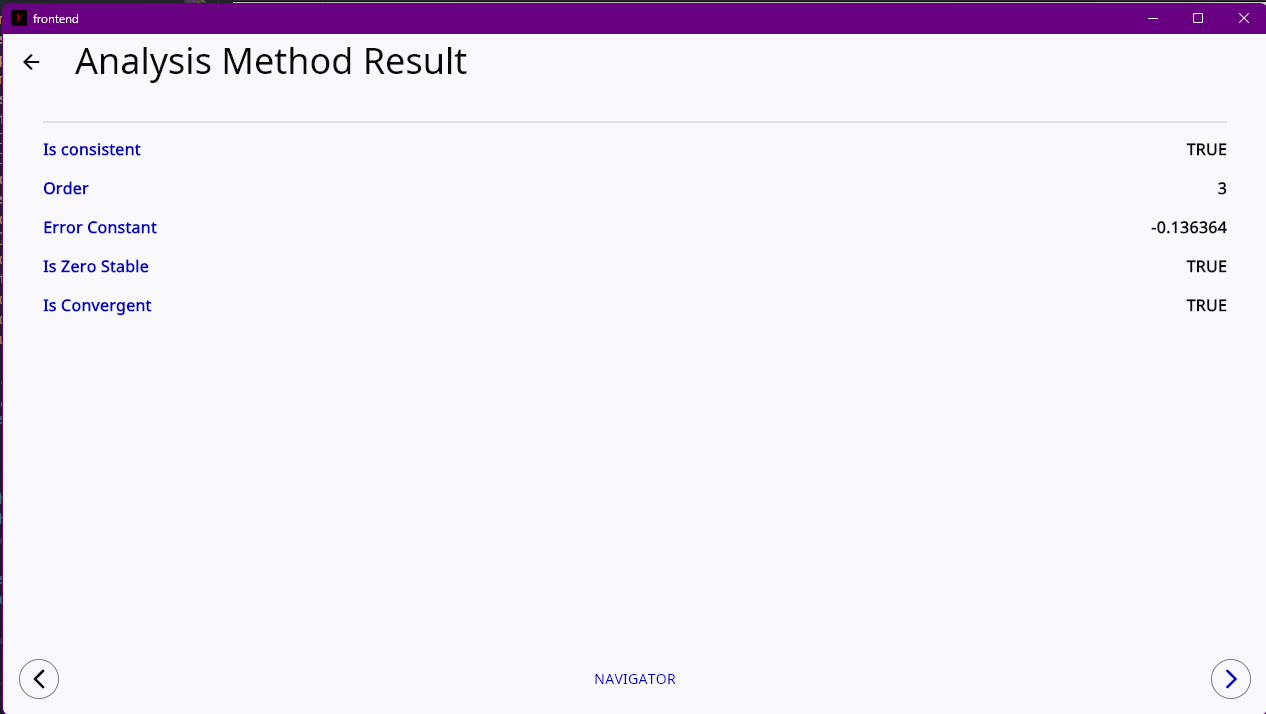
\includegraphics[width=1\textwidth]{chapters/4/image/stiifa.png}
    \caption{Analysis result of $(4.37)$ }
\end{figure}


\begin{figure}[htbp]
    \centering
    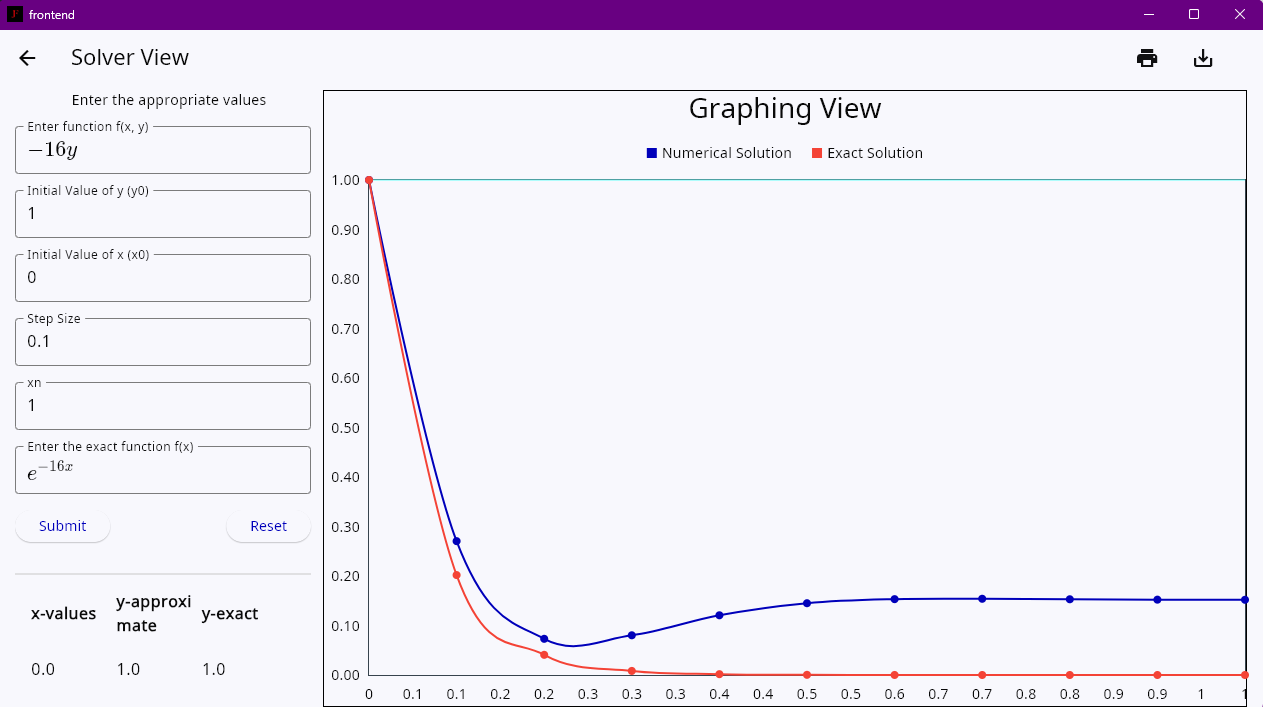
\includegraphics[width=1\textwidth]{chapters/4/image/stiffb.png}
    \caption{solution of $(4.37)$ by JF-Solver}
\end{figure}

\newpage
In conclusion, the numerical examples provided in this chapter effectively demonstrate the accuracy and robustness of the proposed solver across various methods and scenarios. The detailed analysis of Quade's method, Adams family methods, and the 3-step Backward Differentiation Formula showcases the solver's capability in handling both explicit and implicit differential equations. The results, corroborated by theoretical analysis and the use of the JF-Solver software, affirm the solver's reliability and efficiency in practical applications. This comprehensive evaluation highlights the solver's suitability for a wide range of differential equation problems, validating its potential as a valuable tool in numerical analysis.

